
% DIAGRAM (MATTHIAS NOTES)
% -----------------------
\chapter{Non-singlet Vector and Axialvector Correlators}

% definitions 
% -----------
\section{Introduction}
In this chapter we want to investigate the dimension-6 operator product expansion (OPE) contributions to the two-point correlation functions $\Pi^{V/A}_{\mu\nu}(q)$ of non-singlet vector and axialvector currents $j^V_\mu(x) = (\bar u \gamma_\mu d)(x)$ and $j^A_\mu(x)=(\bar u \gamma_\mu \gamma_5 d)(x)$. For simplicity we will only assume massless light quarks (u,d and s) in which case the correlators take the form
\begin{equation}
	\Pi_{\mu\nu}^{V/A}(q) \,\equiv\, i\!\int\! {\rm d}x\, {\rm e}^{iqx}\,
	\langle\Omega|T\{ j_\mu^{V/A}(x) j_\nu^{V/A}(0)^\dagger\}|\Omega\rangle
	\,=\, \big( q_\mu q_\nu - g_{\mu\nu} q^2 \big )\, \Pi^{V/A}(q^2) \,.
\end{equation}
Here $|\Omega\rangle$ denotes the full QCD vacuum and the second identity holds since the vector current is conserved, i.e. $\partial^\mu j_\mu(x) = 0$ and thus $q^\mu \Pi_{\mu\nu}(q^2)$ has to vanish, which implies the Lorentz-structure on the right.
\par
In the framework of the OPE the scalar function $\Pi^{V/A}$ then permits an expansion in powers of $1/Q^2$ with $Q^2\equiv-q^2$
\begin{equation}
	\label{ope}
	\Pi^{V/A}(Q^2) \,=\, C_0(Q^2) + C_4(Q^2)\, \frac{\langle O_4 \rangle}{Q^4} +
	C_6^{V/A}(Q^2)\, \frac{\langle O_6 \rangle}{Q^6} + \ldots \,.
\end{equation}
In the OPE only the Wilson coefficients $C^{V/A}_i$ depend on the momentum, the operators $O_i$ are local, but both depend on the renormalisation scale $\mu$.
\par
Our main concern is to find the contributions of the dimension-6 term, which receives contributions from the three-gluon condensate $\langle g^3 f_{abc} G^a_{\mu\nu} G^{b\nu}_{\lambda} G^{c\lambda \mu} \rangle$ and the quark-condensates. Due to the fact, that the three gluon condensate does not arise at leading order, we will concentrate on four-quark condensates. The contribution of the four-quark condensates has been calculated in \cite{ac94} and \cite{lsc86}. To present it for the V-A and V+A correlation functions we need to transform it into another basis. In general we have chosen our basis, because in the V-A contribution the penguin diagrams cancel each other and we only have to regard the current-current diagrams. In the lowest order of perturbation theory the contributions of the 4-quark operators are well-known and read \cite{svz79}
\begin{equation}
	\label{eq:C6VQ6L}
	\frac{C^{i,V}_6 Q^i_6}{g^2} = -\frac{2}{9}(\bar u \gamma_\mu t^a u + \bar d \gamma_\mu t^a d) \sum_{q=u,d,s} (\bar q \gamma^\mu t^a q) - 2 \bar u \gamma_5 \gamma_\mu t^a d \bar d \gamma_5 \gamma_\mu t^a u
\end{equation}
for the vector correlator and
\begin{equation}
	\label{eq:C6AQ6L}
	\frac{C^{i,A}_6 Q^i_6}{g^2} = -\frac{2}{9}(\bar u \gamma_\mu t^a u + \bar d \gamma_\mu t^a d) \sum_{q=u,d,s} (\bar q \gamma^\mu t^a q) - 2 \bar u \gamma_\mu t^a d \bar d \gamma_\mu t^a u
\end{equation}
for the axial vector one. 
To shorten the equations we want to give the from us used basis of four-quark operators, given by
\begin{eqnarray}
	\label{Qbasis}
	Q_V^{\,o} \,&=&\, (\bar u\gamma_\mu t^a d\bar d\gamma^\mu t^a u) \,, \quad
	Q_A^{\,o} \,=\, (\bar u\gamma_\mu\gamma_5 t^a d\bar d\gamma^\mu\gamma_5 t^a u)
	\,,\\
	\tvs
	Q_V^{\,s} \,&=&\, (\bar u\gamma_\mu d\bar d\gamma^\mu u) \,, \quad
	Q_A^{\,s} \,=\, (\bar u\gamma_\mu\gamma_5 d\bar d\gamma^\mu\gamma_5 u) \,, \\
	\tvs
	Q_3 \,&\equiv&\, (\bar u\gamma_\mu t^a u + \bar d\gamma_\mu t^a d)
	\!\sum\limits_{q=u,d,s} (\bar q\gamma^\mu t^a q) \,, \\
	\tvs
	Q_4 \,&\equiv&\, (\bar u\gamma_\mu\gamma_5 t^a u +
	                  \bar d\gamma_\mu\gamma_5 t^a d)
	\!\sum\limits_{q=u,d,s} (\bar q\gamma^\mu\gamma_5 t^a q) \,, \\
	\tvs
	Q_5 \,&\equiv&\, (\bar u\gamma_\mu u + \bar d\gamma_\mu d)
	\!\sum\limits_{q=u,d,s} (\bar q\gamma^\mu q) \,, \\
	\tvs
	Q_6 \,&\equiv&\, (\bar u\gamma_\mu\gamma_5 u + \bar d\gamma_\mu\gamma_5 d)
	\!\sum\limits_{q=u,d,s} (\bar q\gamma^\mu\gamma_5 q) \,, \\
	\tvs
	Q_7 \,&\equiv&\, \sum\limits_{q=u,d,s} (\bar q\gamma_\mu t^a q)
	\!\sum\limits_{q^\prime=u,d,s} (\bar q^\prime\gamma^\mu t^a q^\prime) \,, \\
	\tvs
	Q_8 \,&\equiv&\, \sum\limits_{q=u,d,s} (\bar q\gamma_\mu\gamma_5 t^a q)
	\!\sum\limits_{q^\prime=u,d,s} (\bar q^\prime\gamma^\mu\gamma_5 t^a q^\prime)
	\,, \\
	\tvs
	Q_9 \,&\equiv&\, \sum\limits_{q=u,d,s} (\bar q\gamma_\mu q)
	\!\sum\limits_{q^\prime=u,d,s} (\bar q^\prime\gamma^\mu q^\prime) \,, \\
	\tvs
	Q_{10} \,&\equiv&\, \sum\limits_{q=u,d,s} (\bar q\gamma_\mu\gamma_5 q)
	\!\sum\limits_{q^\prime=u,d,s} (\bar q^\prime\gamma^\mu\gamma_5 q^\prime) \,.
\end{eqnarray} 
where $Q^O_{V/A}$ $Q^S_{V/A}$ are termed current-current operators and $Q_3$ to $Q_{10}$ penguin operators. In addition we have defined the four current-current operators
\begin{equation}
	Q^O_\pm = Q^O_V \pm Q^O_A \qquad \text{and} \qquad Q^S_\pm \equiv Q^S_V \pm Q^S_A.
\end{equation}
\par
The explicit calculation of the one-loop corrections to 4-quark condensates in eq.~(\ref{eq:C6VQ6L}) and (\ref{eq:C6AQ6L}) gives \cite{lsc86}
\begin{equation}
	\begin{split}
		\frac{C^{i,V}Q^i_6}{g^2} &= -\frac{2}{9}\left(1 + a_s \left[\frac{95}{72}L + \frac{107}{48}\right]\right) Q_3 \\
		& - \frac{1}{3}\left(1 + a_s \left[\frac{9}{8}L + \frac{431}{96} \right] \right) O^{o,A}_1 \\
		&- \frac{a_s}{24\pi} \left[ (16L - 12) Q^s_V + \left(30 L - \frac{45}{2}\right) Q^o_V + \left(\frac{16}{9} L - \frac{8}{27} \right) Q_7  \right. \\
		&+ \left. \left(\frac{16}{9} L + \frac{56}{27} \right) Q_6 + \left(\frac{10}{3}L + \frac{35}{9} \right)Q_4\right],
	\end{split}
\end{equation} 
where we used the operator $O^{o,A}_1$ defined as
\begin{equation}
	O^{o,A}_1 = \bar u \Gamma^{[3]} t^a d \bar d \Gamma^{[3]} t^a u.
\end{equation}
For the axial vector correlator the corrections look exactly the same, except for the matrices displayed below change into
\begin{equation}
	\begin{split}
		O^{o,A}_1 &\rightarrow O^{o,V}_1 \\,
		Q^s_V &\rightarrow Q^s_A \\,
		Q^o_V &\rightarrow Q^o_a.
	\end{split}
\end{equation}
Thus using a short Mathematica script (app.~(\ref{lst:MathematicaDim6Ope}))  we can transform the one-loop corrections to 4-quark condensates into the from us needed basis 
\begin{equation}
	\label{C6O6VmA}
	C_6^{V-A}(Q^2)\,\langle O_6 \rangle \,=\,
	4\pi^2 a_s \,\Big\{ \Big[\, 2 + \Big( \sfrac{25}{6} - L \Big ) a_s \Big]
	\langle Q_-^{\,o} \rangle -
	\Big( \sfrac{11}{18} - \sfrac{2}{3} L \Big ) a_s \langle Q_-^{\,s} \rangle
	\Big\} \,,
\end{equation}
and
\begin{eqnarray}
	C_6^{V+A}(Q^2)\,\langle O_6 \rangle \,&=&\,
	-\,4\pi^2 a_s \,\Big\{ \Big[\, 2 + \Big( \sfrac{155}{24} - \sfrac{7}{2} L \Big )
	a_s \Big] \langle Q_+^{\,o} \rangle +
	\Big( \sfrac{11}{18} - \sfrac{2}{3} L \Big ) a_s \langle Q_+^{\,s} \rangle +
	\nn \\
	\mvs
	&& \hspace{17mm}
	\Big[\, \sfrac{4}{9} + \Big( \sfrac{37}{36} - \sfrac{95}{162} L \Big ) a_s \Big]
	\langle Q_3 \rangle +
	\Big( \sfrac{35}{108} - \sfrac{5}{18} L \Big ) a_s \langle Q_4 \rangle + \nn \\
	\mvs
	&& \hspace{27mm}
	\label{C6O6VpA}
	\Big( \sfrac{14}{81} - \sfrac{4}{27} L \Big ) a_s \langle Q_6 \rangle -
	\Big( \sfrac{2}{81} + \sfrac{4}{27} L \Big ) a_s \langle Q_7 \rangle \,,
\end{eqnarray}
where $a_s=\alpha_s/\pi$ and $L\equiv \ln Q^2/\mu^2$. 
\par
\par
Before continuing with the calculation of the anomalous dimension matrix $\hat \gamma_O$ we want to investigate the scale dependence of a general term $R_O$ in the OPE, corresponding to a set of operators $\vec O(\mu)$
\begin{equation}
	R_O = \vec R^T (\mu) \langle \vec O(\mu) \rangle,
\end{equation}
where we displayed the dependency on the scale $\mu$ explicitly and the dependence on other potential dimensionful parameters implicitly. Due to the fact, that for the vector and axialvector currents renormalisation scale dependence only arises from pertubative contributions, $R_O$ should not be dependent on the scale $\mu$ and we can write
\begin{equation}
	\label{eq:ROMuIndependent}
	\left[\mu \frac{d}{d\mu} \vec C^T(\mu) \right] \langle \vec O (\mu) \rangle = -C^T (\mu) \left[\mu \frac{d}{d\mu} \langle \vec O (\mu) \rangle \right]
\end{equation}
Furthermore the anomalous dimension matrix $\hat \gamma_O$ of the operator matrix can be defined by
\begin{equation}
	\label{eq:anomalousDimensionMatrix}
	-\mu\frac{d}{d\mu} \langle \vec O(\mu) \rangle \equiv \hat \gamma_O(a_\mu) \langle \vec O(\mu) \rangle 
\end{equation},
where $a_\mu = a_s(\mu)$.
Plugging in eq.~(\ref{eq:ROMuIndependent}) into eq.~(\ref{eq:anomalousDimensionMatrix}) and transposing the matrices one obtains the RGE that has to be satisfied by the coefficient function $\vec C(\mu)$.
\begin{equation}
	\label{eq:rgeCheck}
	\mu\frac{d}{d\mu} \vec C(\mu) = \hat \gamma^T_O(a_\mu) \vec C(\mu).
\end{equation}
This equation shall be checked for the coefficient functions of the dimension-6 operators in eqs.(\ref{C6O6VmA}) and (\ref{C6O6VpA}). 
\par
Hereafter we want to calculate the anomalous dimension matrices for the cases V-A and V+A, before we continue with checking the RGE for each of them.

\section{4-point Green's Function With Operator Insertion}
	To show the basic calculation method we want to start by calculating the most accessible diagram. We will use the first two operators of our proposed basis in eq.~(\ref{Qbasis}), given by 
	\begin{equation}
		\label{eq:4QuarkOperators}
		Q^S_{V,A} = \left ( \bar{q}^A \Gamma_1 q^B \bar q^B \Gamma_2 q^A \right )  (z) \qquad \text{ and } \qquad  Q^O_{V,A} = \left ( \bar{q}^A t^a \Gamma_1 q^B \bar q^B t^a \Gamma_2 q^A \right )  (z), 
	\end{equation}			
	\begin{equation}
		Q_- = Q_{V-A} = Q^{S,O}_{V} - Q^{S,O}_{A}
	\end{equation}
	where A and B denote flavor indices. Additionally $Q^S_{V,A}$ stands for the singlet operator and $Q^O_{V,A}$ for the octet operator (the octet operator contains the color matrix $t^a$). The indices $V,A$ denote the structure of the operators, which can be either vector ($\gamma_\mu$) or axialvector ($\gamma_\mu\gamma_5$). $\Gamma_1$ and $\Gamma_2$ are equal 4x4 matrices and will be replaced later by vector $\gamma_\mu$  or axial-vector $\gamma_\mu \gamma_5$ structure.  
\par 
To show the principles of the calculation method we will be very explicit within the first computation. Starting with the construction of a 4-point Green's function we need to add four external fields 
	\begin{equation}
		\bar q_\alpha^i (x_1) q_\beta^j (x_2) \bar q_\delta^k (x_3) q_\gamma^l (x_4),
	\end{equation}
	where $i,j,k,l$ denote color-indices and $\alpha, \beta, \delta, \gamma$ stand for Dirac-indices. Then the general definition of the 4-point Green's function is given by 
	\begin{equation}
		\label{eq:fourQuarkGreensFunction}
		\begin{split}
			\Gamma &= \int d^Dx_1d^Dx_2d^Dx_3d^Dx_4 e^{i(p_1x_1+p_2x_2+p_3x_3+p_4x_4)} \\	
			&\times \langle 0 | T  \{ \bar q_\alpha^i (x_1) q_\beta^j (x_2) \bar q_\delta^k (x_3) q_\gamma^l (x_4) e^{i\int d^Dz \mathcal{L}_I(z)} \}  | 0  \rangle, 
		\end{split}
	\end{equation}
	where the interaction term ($e^{i\int d^Dz \mathcal{L}_I(z)}$) is equal to one for the zeroth-order calculation. Now inserting our first operator from eq.~(\ref{eq:4QuarkOperators}) yields
	\begin{equation*}
		\begin{split}
			\Gamma^0 &= \int d^D x_1 d^D x_2 d^D x_3 d^D x_4 d^Dz e^{i(p_1x_1 + p_2x_2 + p_3x_3 + p_4x_4)} \\ 
			  &\times  \langle 0  |T\{ q_\alpha^i(x_1) \bar q_\beta^j(x_2) [ \bar q^A t^a\Gamma_1 q^B \bar q^B t^a\Gamma_2 q^A ](z) q_\delta^k(x_3) \bar q_\gamma^l(x_4) \}  |0 \rangle \\ 
			&= (-1)^4 \int d^D x_1 d^D x_2 d^D x_3 d^D x_4 d^Dz e^{i(p_1x_1 + p_2x_2 + p_3x_3 + p_4x_4)} \\ 
			&\times  \langle 0  | T \{ q_\alpha^i(x_1) \bar q^A(z) t^a\Gamma_1 q^B(z) \bar q_\beta^j(x_2) q_\delta^k(x_3) \bar q^B(z) t^a\Gamma_2 q^A(z) \bar q_\gamma^l(x_4) \}  | 0  \rangle, 
		\end{split}
	\end{equation*}
	where we had to perform four permutations in the last line. Every permutation yields a factor of $-1$, due to the anti-commutating characteristics of the Dirac-fields.
	\begin{equation}
		 q_\alpha \bar q_\beta = (-1) \bar q_\beta q_\alpha	
	\end{equation}
	Using Wick's theorem and the propagator relation eq.~\ref{eq:quarkPropagator} we now want to contract the fields. Hence regarding only the time-ordered part 
	\begin{equation*}
		\begin{split}
			\Gamma^0 &= \int d^D x_1 d^D x_2 d^D x_3 d^D x_4 dz e^{i(p_1x_1 + p_2x_2 + p_3x_3 + p_4x_4)} \\ 
			&\cdot  \langle 0  | T \{ 
			\contraction[2ex]{}{q}{{}_\alpha^i(x_1) \bar}{q} 
			q_\alpha^i(x_1) \bar q^A(z) t^a\Gamma_1 
			\contraction[2ex]{}{q}{{}^B(z) \bar}{q}
			q^B(z) \bar q_\beta^j(x_2) 
			\contraction[2ex]{}{q}{{}_\delta^k(x_3) \bar}{q}
			q_\delta^k(x_3) \bar q^B(z) t^a\Gamma_2 
			\contraction[2ex]{}{q}{{}^A(z) \bar}{q}
			q^A(z) \bar q_\gamma^l(x_4) \}  | 0  \rangle \\
			 &= \delta^{ij}\delta^{kl}(i)^4 \int d^D x_1 d^D x_2 d^D x_3 d^D x_4 dz e^{i(p_1x_1 + p_2x_2 + p_3x_3 + p_4x_4)} \\ 
			&\cdot [S^A(x_1-z) t^a\Gamma_1 S^B(z-x_2) ]_{\alpha\beta} [S^B(x_3-z)t^a\Gamma_2S^A(z-x_4)]_{\delta\gamma},
		\end{split}
	\end{equation*}
	The two Kronecker deltas ($\delta^{ij}, \delta^{kl}$) rise from color conservation between the in- and outgoing quarks and the factor $(i)^4$ is obtained from contraction forming the quark-propagator eq.~(\ref{eq:quarkPropagator}).  \par
	Now we want to perform a Fourier-transformation. As we are not facing a loop, all integrals are supposed to vanish. Transforming all four propagators gives
	\begin{equation}
		\begin{split}
			S^A(x_1-z) &= \int \frac{d^Dk_1}{(2\pi)^D} e^{-ik_1(x_1-z)} S^A(k_1) \\
			S^B(z-x_2) &= \int \frac{d^Dk_2}{(2\pi)^D} e^{-ik_2(z-x_2)} S^B(k_2) \\
			S^B(x_3-z) &= \int \frac{d^Dk_3}{(2\pi)^D} e^{-ik_3(x_3-z)} S^B(k_3) \\
			S^A(z-x_4) &= \int \frac{d^Dk_4}{(2\pi)^D} e^{-ik_4(z-x_4)} S^A(k_4). 
		\end{split}
	\end{equation}
	Inserting the above relations into $\Gamma_0$ yields
	\begin{equation}
		\begin{split}
			\Gamma^0
			 &= \delta^{ij}\delta^{kl} \int d^D x_1 d^D x_2 d^D x_3 d^D x_4 dz \frac{d^D k_1}{(2\pi)^D} \frac{d^D k_2}{(2\pi)^D} \frac{d^D k_3}{(2\pi)^D} \frac{d^D k_4}{(2\pi)^D} \\
			&\cdot e^{-ik_1(x_1-z)} e^{-ik_2(z-x_2)}e^{-ik_3(x_3-z)}e^{-ik_4(z-x_4)} e^{i(p_1x_1 + p_2x_2 + p_3x_3 + p_4x_4)} \\ 
			&\cdot [S^A(k_1) t^a\Gamma_1 S^B(k_2) ]_{\alpha\beta} [S^B(k_3)t^a\Gamma_2S^A(k_4)]_{\delta\gamma}.
		\end{split}
	\end{equation}
	Reordering the exponential function and integrating over $dx_1, dx_2, dx_3, dx_4$ and $d^Dz$ will give us the needed Dirac delta distributions
	\begin{equation}
		\begin{split}
			\Gamma_0 &= \delta^{ij}\delta^{kl} \int d^D x_1 d^D x_2 d^D x_3 d^D x_4 dz \frac{d^D k_1}{(2\pi)^D} \frac{d^D k_2}{(2\pi)^D} \frac{d^D k_3}{(2\pi)^D} \frac{d^D k_4}{(2\pi)^D} \\
			&\cdot e^{ix_1(p_1-k_1)} e^{ix_2(p_2+k_2)} e^{ix_3(p_3-k_3)} e^{ix_4(p_4+k_4)} e^{iz(k_1+k_3-k_2-k_4)} \\
			&\cdot [S^A(k_1) t^a\Gamma_1 S^B(k_2) ]_{\alpha\beta} [S^B(k_3)t^a\Gamma_2S^A(k_4)]_{\delta\gamma} \\
			 &= \delta^{ij}\delta^{kl} \int d^D x_1 d^D x_2 d^D x_3 d^D x_4 dz \frac{d^D k_1}{(2\pi)^D} \frac{d^D k_2}{(2\pi)^D} \frac{d^D k_3}{(2\pi)^D} \frac{d^D k_4}{(2\pi)^D} \\
			&\cdot \delta^{(D)}(p_1-k_1) \delta^{(D)}(p_2+k_2) \delta^{(D)}(p_3-k_3) \delta^{(D)}(p_4+k_4) \delta^{(D)}(k_1+k_3-k_2-k_4) \\
			&\cdot [S^A(k_1) t^a\Gamma_1 S^B(k_2) ]_{\alpha\beta} [S^B(k_3)t^a\Gamma_2S^A(k_4)]_{\delta\gamma}.
		\end{split}
	\end{equation}
	Integrating over $k_1, k_2, k_3$ and $k_4$ gives us the following relations due to the Dirac-deltas
	\begin{equation}
		\begin{split}
			k_1 = p_1, \qquad k_2 = -p_2, \qquad k_3 = p_3, \qquad k_4 = -p_4, \qquad k_1 + k_3 = k_2 + k_4, 
		\end{split}
	\end{equation}
	The last relation has been contributed from the z integration and represents the impulse conservation of the in-going ($p_1, p_3$) and outgoing ($p_2, p_4$) impulses. Thus we are left with
	\begin{equation}
		\begin{split}
			\Gamma_0 &= \delta^{ij}\delta^{kl} [S^A(-p_1) t^a\Gamma_1 S^B(p_2) ]_{\alpha\beta} [S^B(-p_3)t^a\Gamma_2S^A(p_4)]_{\delta\gamma},
		\end{split}
	\end{equation}
	which can be displayed as a Feynman diagram
	\vspace{0.5cm}
	\begin{fmffile}{samplepics}
		\begin{equation}
		\begin{gathered}
		\begin{fmfgraph*}(100,75)
			\fmfleftn{i}{2} \fmfrightn{o}{2}
			\fmf{fermion, label=$p_3$}{i1,v1}
			\fmf{fermion, label=$p_4$, label.side=right}{v1,o1}
			\fmf{fermion, label=$p_1$, label.side=left}{i2,v1}
			\fmf{fermion, label=$p_2$}{v1,o2}
			\fmfv{decoration.shape=square, decoration.size=6, label=z}{v1}
			\fmflabel{$x_1$}{i2}
			\fmflabel{$x_3$}{i1}
			\fmflabel{$x_2$}{o2}
			\fmflabel{$x_4$}{o1}
		\end{fmfgraph*}
		\end{gathered}
		=	
		\bcontraction[1ex]{}{q}{{}^i_\alpha(x_1) \bar q^j_\beta(x_2) [ \bar}{q} 
		\contraction[1ex]{q^i_\alpha(x_1) \bar}{q}{{}^j_\beta(x_2) [ \bar q^A \Gamma_1}{q}
		q^i_\alpha(x_1) \bar q^j_\beta(x_2) [ \bar q^A \Gamma_1 q^B 
		\bcontraction[1ex]{\bar}{q}{{}^B \Gamma_2 q^A ](z)}{q}
		\contraction[1ex]{\bar q^B \Gamma_2}{q}{{}^A ](z) q^k_\delta(x_3) \bar}{q}
		\bar q^B \Gamma_2 q^A ](z) q^k_\delta(x_3) \bar q^l_\gamma(x_4).
		\end{equation}
	\end{fmffile}
		
	Amputating the external-propagators will give us the zeroth-order structures. Hence for the singlet operator $Q^S_{V,A}$ we get a contribution of
	\begin{equation}
		 \Gamma^{0,S}_{amp} = \delta^{ij}\delta^{kl}[\Gamma_1]^{AB}_{\alpha\beta}[\Gamma_2]^{BA}_{\delta\gamma}
	\end{equation}
	and for the octet operator $Q^O_{V,A}$ we get 
	\begin{equation}
		\Gamma^{0,O}_{amp} = (t^a)^{ij}(t^a)^{kl}[\Gamma_1]^{AB}_{\alpha\beta}[\Gamma_2]^{BA}_{\delta\gamma}
	\end{equation} 
	\newpage

	\section{V-A Current-current Diagram Contributions} 
	Having understood the basic calculation method we now want to deal with first-order diagrams, concentrating on the quark-gluon interactions. Remembering the definition of our four quark Green's function eq.~(\ref{eq:fourQuarkGreensFunction}) we need to expand the interaction term in the exponential function
	\begin{equation}
		\begin{split}
			e^x &= 1 + x + \frac{x^2}{2!} + \frac{x^3}{3!} + ... \\
			e^{i\int d^D z \mathcal{L}_I(z)} &= 1 + g_sB_a^\mu(x)\sum_f\bar q_f^\alpha \gamma^\mu (t^a)_{\alpha\beta}q_f^\beta \\
			&+ \frac{g_s^2}{2} [B_a^\mu(x)\sum_f\bar q_f^\alpha \gamma^\mu (t^a)_{\alpha\beta}q_f^\beta] [B_b^\nu(x)\sum_f\bar q_f^\sigma \gamma^\nu (t^b)_{\sigma\delta}q_f^\delta]  + \ldots , 
		\end{split}
	\end{equation}
	which will give us the following possible contractions 
	\begin{equation}
		a) = 
%		-------------------------
		\contraction{}{q}{{}^i_\alpha(x_1) \bar q^j_\beta(x_2) [ \bar q^A \Gamma_1 q^B \bar q^B \Gamma_2 q^A ](z) [ B^\lambda_b \bar}{q}
		\bcontraction{q^i_\alpha(x_1) \bar}{q}{{}^j_\beta(x_2)[ \bar q^A \Gamma_1 q^B \bar q^B \Gamma_2 q^A ](z) [ B^\lambda_c \bar q \gamma_\lambda t^c q ](y_1) [ B^\sigma_b \bar q \gamma_\sigma t^c }{q}
		\contraction[2ex]{q^i_\alpha(x_1) \bar q^j_\beta(x_2) [ \bar}{q}{^A \Gamma_1 q^B \bar q^B \Gamma_2 q^A ](z) [ B^\lambda_b \bar q \gamma_\lambda t^b }{q}
		\bcontraction[2ex]{q^i_\alpha(x_1) \bar q^j_\beta(x_2) [ \bar q^A \Gamma_1 }{q}{{}^B \bar q^B \Gamma_2 q^A ](z) [ B^\lambda_b \bar}{q}
		\contraction[3ex]{q^i_\alpha(x_1) \bar q^j_\beta(x_2) [ \bar q^A \Gamma_1 q^B \bar }{q}{{}^B \Gamma_2 q^A ](z) [ B^\lambda_b \bar q \gamma_\lambda t^b q ](y_1) [ B^\sigma_c \bar q \gamma_\sigma t^c q ](y_2) }{q}
		\bcontraction[3ex]{q^i_\alpha(x_1) \bar q^j_\beta(x_2) [ \bar q^A \Gamma_1 q^B \bar q^B \Gamma_2}{q}{{}^A ](z) [ B^\lambda_b \bar q \gamma_\lambda t^b q ](y_1) [ B^\sigma_c \bar q \gamma_\sigma t^c q ](y_2) q^k_\delta (x_3) \bar }{q}
		\contraction[4ex]{q^i_\alpha(x_1) \bar q^j_\beta(x_2) [ \bar q^A \Gamma_1 q^B \bar q^B \Gamma_2 q^A ](z) [ }{B}{{}^\lambda_b \bar q \gamma_\lambda t^b q ](y_1) [ }{B}
% 		---------------------------------
		q^i_\alpha(x_1) \bar q^j_\beta(x_2) [ \bar q^A \Gamma_1 q^B \bar q^B \Gamma_2 q^A ](z) [ B^\lambda_b \bar q \gamma_\lambda t^b q ](y_1) [ B^\sigma_c \bar q \gamma_\sigma t^c q ](y_2) q^k_\delta (x_3) \bar q^l_\gamma (x_4),
	\end{equation}

	\begin{equation}
		\label{eq:NormalContractionB}
		b) = 
%		-------------------------
		\contraction{}{q}{(x_1) \bar q(x_2) [\bar}{q}
		\bcontraction{q(x_1) \bar}{q}{(x_2) [\bar q}{q}
		\contraction[2ex]{q(x_1) \bar q(x_2) [\bar q q \bar }{q}{q](z) q(x_3) \bar q(x_4) [B \bar q}{q}
		\bcontraction[3ex]{q(x_1) \bar q(x_2) [\bar q q \bar q}{q}{](z) q(x_3) \bar q(x_4) [B \bar q q](y_1) [B \bar }{q}
		\contraction{q(x_1) \bar q(x_2) [\bar q q \bar q q](z) }{q}{(x_3) \bar q(x_4) [B \bar }{q}
		\bcontraction[2ex]{q(x_1) \bar q(x_2) [\bar q q \bar q q](z) q(x_3) \bar }{q}{(x_4) [B \bar q q](y_1) [B \bar q}{q}
		\bcontraction{q(x_1) \bar q(x_2) [\bar q q \bar q q](z) q(x_3) \bar q(x_4) [}{B}{ \bar q q](y_1) [}{B}
% 		---------------------------------
		q(x_1) \bar q(x_2) [\bar q q \bar q q](z) q(x_3) \bar q(x_4) [B \bar q q](y_1) [B \bar q q](y_2) ,
	\end{equation}

	\begin{equation}
		c) = 
%		-------------------------
		\contraction[3ex]{}{q}{(x_1) \bar q(x_2) [\bar q q \bar q q](z) q(x_3) \bar q(x_4) [B \bar }{q}
		\contraction{q(x_1) \bar}{q}{(x_2) [\bar q}{q}
		\bcontraction[2ex]{q(x_1) \bar q(x_2) [\bar }{q}{q \bar q q](z) q(x_3) \bar q(x_4) [B \bar q}{q}
		\contraction[2ex]{q(x_1) \bar q(x_2) [\bar q q \bar }{q}{q](z) q(x_3) \bar q(x_4) [B \bar q q](y_1) [B \bar q}{q}
		\contraction{q(x_1) \bar q(x_2) [\bar q q \bar q}{q}{](z) q(x_3) \bar }{q}
		\bcontraction{q(x_1) \bar q(x_2) [\bar q q \bar q q](z) }{q}{(x_3) \bar q(x_4) [B \bar q q](y_1) [B \bar }{q}
		\contraction{q(x_1) \bar q(x_2) [\bar q q \bar q q](z) q(x_3) \bar q(x_4) [}{B}{ \bar q q](y_1) [}{B}
% 		---------------------------------
		q(x_1) \bar q(x_2) [\bar q q \bar q q](z) q(x_3) \bar q(x_4) [B \bar q q](y_1) [B \bar q q](y_2) ,
	\end{equation}

	\begin{equation}
		d) = 
%		-------------------------
		\contraction{}{q}{(x_1) \bar q(x_2) [\bar }{q}
		\bcontraction[2ex]{q(x_1) \bar }{q}{(x_2) [\bar q q \bar q q](z) q(x_3) \bar q(x_4) [B \bar q}{q}
		\contraction[3ex]{q(x_1) \bar q(x_2) [\bar q}{q}{\bar q q](z) q(x_3) \bar q(x_4) [B \bar }{q}
		\contraction[2ex]{q(x_1) \bar q(x_2) [\bar q q \bar}{q}{q](z) }{q}
		\contraction{q(x_1) \bar q(x_2) [\bar q q \bar q}{q}{](z) q(x_3) \bar q(x_4) [B \bar q q](y_1) [B \bar }{q}
		\bcontraction{q(x_1) \bar q(x_2) [\bar q q \bar q q](z) q(x_3) \bar }{q}{(x_4) [B \bar q q](y_1) [B \bar q }{q}
		\contraction{q(x_1) \bar q(x_2) [\bar q q \bar q q](z) q(x_3) \bar q(x_4) [}{B}{\bar q q](y_1) [}{B}
% 		---------------------------------
		q(x_1) \bar q(x_2) [\bar q q \bar q q](z) q(x_3) \bar q(x_4) [B \bar q q](y_1) [B \bar q q](y_2), 
	\end{equation}

	\begin{equation}
		e) = 
%		-------------------------
		\contraction[2ex]{}{q}{(x_1) \bar q(x_2) [\bar q q \bar q q](z) q(x_3) \bar q(x_4) [B \bar }{q}
		\contraction{q(x_1) \bar }{q}{(x_2) [\bar q}{q}
		\contraction{q(x_1) \bar q(x_2) [\bar q q \bar }{q}{q](z)}{q}
		\bcontraction{q(x_1) \bar q(x_2) [\bar q q \bar q}{q}{](z) q(x_3) \bar q(x_4) [B \bar q q](y_1) [B \bar }{q}
		\contraction{q(x_1) \bar q(x_2) [\bar q q \bar q q](z) q(x_3) \bar }{q}{(x_4) [B \bar q q](y_1) [B \bar q }{q}
		\bcontraction[2ex]{q(x_1) \bar q(x_2) [\bar q q \bar q q](z) q(x_3) \bar q(x_4) [}{B}{\bar q q](y_1) [}{B}
% 		---------------------------------
		q(x_1) \bar q(x_2) [\bar q q \bar q q](z) q(x_3) \bar q(x_4) [B \bar q q](y_1) [B \bar q q](y_2), 
	\end{equation}
	
	\begin{equation}
		f) = 
%		-------------------------
		\contraction[1ex]{}{q}{(x_1) \bar q(x_2) [\bar }{q}
		\bcontraction[3ex]{q(x_1) \bar }{q}{(x_2) [\bar q q \bar q q](z) q(x_3) \bar q(x_4) [B \bar q }{q}
		\bcontraction[2ex]{q(x_1) \bar q(x_2) [\bar q }{q}{\bar q q](z) q(x_3) \bar q(x_4) [B \bar }{q}
		\contraction[2ex]{q(x_1) \bar q(x_2) [\bar q q \bar }{q}{q](z) q(x_3) \bar q(x_4) [B \bar q q](y_1) [B \bar q }{q}
		\contraction{q(x_1) \bar q(x_2) [\bar q q \bar q }{q}{](z) q(x_3) \bar }{q}
		\bcontraction{q(x_1) \bar q(x_2) [\bar q q \bar q q](z)}{q}{(x_3) \bar q(x_4) [B \bar q q](y_1) [B \bar }{q}
		\contraction{q(x_1) \bar q(x_2) [\bar q q \bar q q](z) q(x_3) \bar q(x_4) [}{B}{\bar q q](y_1) [}{B}
% 		---------------------------------
		q(x_1) \bar q(x_2) [\bar q q \bar q q](z) q(x_3) \bar q(x_4) [B \bar q q](y_1) [B \bar q q](y_2).
	\end{equation}	
	Notice that we only displayed terms needed for the contractions for all diagrams (except for a). In Addition we can draw the former contraction in forms of diagrams 
	\begin{fmffile}{V-ADiagrams}
		\begin{equation}
		a)
		\begin{gathered}
		\begin{fmfgraph}(50,40)
			\fmfleftn{i}{2} \fmfrightn{o}{2}
			\fmf{vanilla, tension=0.5}{i1,z}
			\fmf{vanilla, tension=1.5}{i2,y1}
			\fmf{vanilla, tension=0.7}{y1,z}
			\fmf{vanilla, tension=0.5}{z,o1}
			\fmf{vanilla, tension=0.7}{z,y2}
			\fmf{vanilla, tension=1.5}{y2,o2}
			\fmf{gluon, tension=0}{y1,y2}
		\end{fmfgraph}
		\end{gathered}
		b)
		\begin{gathered}
		\begin{fmfgraph}(50,40)
			\fmfleftn{i}{2} \fmfrightn{o}{2}
			\fmf{vanilla, tension=0.5}{i2,z}
			\fmf{vanilla, tension=0.5}{o2,z}
			\fmf{vanilla, tension=1.5}{i1,y1}	
			\fmf{vanilla, tension=0.7}{y1,z}
			\fmf{vanilla, tension=0.7}{z,y2}
			\fmf{vanilla, tension=1.5}{y2,o1}
			\fmf{gluon, tension=0}{y1,y2}
		\end{fmfgraph}
		\end{gathered}
		c)
		\begin{gathered}
		\begin{fmfgraph}(50,40)
			\fmfleftn{i}{2} \fmfrightn{o}{2}
			\fmf{vanilla, tension=1.5}{i2,y1}
			\fmf{vanilla, tension=0.7}{y1,z}
			\fmf{vanilla, tension=0.5}{z,o2}
			\fmf{vanilla, tension=1.5}{i1,y2}
			\fmf{vanilla, tension=0.7}{y2,z}
			\fmf{vanilla, tension=0.5}{z,o1}
			\fmf{gluon, tension=0}{y1,y2}
		\end{fmfgraph}
		\end{gathered}
		d)
		\begin{gathered}
		\begin{fmfgraph}(50,40)
			\fmfleftn{i}{2} \fmfrightn{o}{2}
			\fmf{vanilla, tension=0.5}{i2,z}
			\fmf{vanilla, tension=0.7}{z,y1}
			\fmf{vanilla, tension=1.5}{y1,o2}
			\fmf{vanilla, tension=0.5}{i1,z}
			\fmf{vanilla, tension=0.7}{z,y2}
			\fmf{vanilla, tension=1.5}{y2,o1}
			\fmf{gluon, tension=0}{y1,y2}
		\end{fmfgraph}
		\end{gathered}
		e)
		\begin{gathered}
		\begin{fmfgraph}(50,40)
			\fmfleftn{i}{2} \fmfrightn{o}{2}
			\fmf{vanilla}{i2,y1}
			\fmf{vanilla}{y1,z}
			\fmf{vanilla}{z,o2}
			\fmf{vanilla}{i1,z}
			\fmf{vanilla}{z,y2}
			\fmf{vanilla}{y2,o1}
			\fmf{gluon, tension=0, left}{y1,y2}
		\end{fmfgraph}
		\end{gathered}
		f)
		\begin{gathered}
		\begin{fmfgraph}(50,40)
			\fmfleftn{i}{2} \fmfrightn{o}{2}
			\fmf{vanilla}{i2,z}
			\fmf{vanilla}{z,y2}
			\fmf{vanilla}{y2,o2}
			\fmf{vanilla}{i1,y1}
			\fmf{vanilla}{y1,z}
			\fmf{vanilla}{z,o1}
			\fmf{gluon, tension=0, left}{y1,y2}
		\end{fmfgraph}
		\end{gathered}.
		\end{equation}
	\end{fmffile}
	Until this point we have only regarded current-current diagrams excluding penguin diagrams. As we will see they later the penguin contributions cancel each others for the $Q_-$ operators. Consequently we will now calculate the contributions of the six current-current diagrams and deal with the penguin diagrams to a later point. \par
	Now we want to calculate the contributions of the anomalous dimension matrix of the six diagrams explicitly (labeled by a,$\ldots$,f). Therefore we will compute their divergencies and consequently their renormalisation constants, which will finally lead with an simple relation to the anomalous dimension matrix of our $Q_-$ operator. 
	\subsection*{Diagram a)}
	Inserting the expanded e-function into the four-quark Green's function eq.~(\ref{eq:fourQuarkGreensFunction}) yields
	\begin{equation}
		\begin{split}
			\Gamma^a &=  g_s^2 \int d^Dx_1d^Dx_2d^Dx_3d^Dx_4d^Dzd^Dy_1d^Dy_2 e^{i(p_1x_1+p_2x_2+p_3x_3+p_4x_4)} \\
				&\cdot \langle 0 | T\{ 
%		-------------------------
			\contraction{}{q}{{}^i_\alpha(x_1) \bar q^j_\beta(x_2) [ \bar q^A \Gamma_1 q^B \bar q^B \Gamma_2 q^A ](z) [ B^\lambda_b \bar}{q}
			\bcontraction{q^i_\alpha(x_1) \bar}{q}{{}^j_\beta(x_2)[ \bar q^A \Gamma_1 q^B \bar q^B \Gamma_2 q^A ](z) [ B^\lambda_c \bar q \gamma_\lambda t^c q ](y_1) [ B^\sigma_b \bar q \gamma_\sigma t^c }{q}
			\contraction[2ex]{q^i_\alpha(x_1) \bar q^j_\beta(x_2) [ \bar}{q}{^A \Gamma_1 q^B \bar q^B \Gamma_2 q^A ](z) [ B^\lambda_b \bar q \gamma_\lambda t^b }{q}
			\bcontraction[2ex]{q^i_\alpha(x_1) \bar q^j_\beta(x_2) [ \bar q^A \Gamma_1 }{q}{{}^B \bar q^B \Gamma_2 q^A ](z) [ B^\lambda_b \bar}{q}
			\contraction[3ex]{q^i_\alpha(x_1) \bar q^j_\beta(x_2) [ \bar q^A \Gamma_1 q^B \bar }{q}{{}^B \Gamma_2 q^A ](z) [ B^\lambda_b \bar q \gamma_\lambda t^b q ](y_1) [ B^\sigma_c \bar q \gamma_\sigma t^c q ](y_2) }{q}
			\bcontraction[3ex]{q^i_\alpha(x_1) \bar q^j_\beta(x_2) [ \bar q^A \Gamma_1 q^B \bar q^B \Gamma_2}{q}{{}^A ](z) [ B^\lambda_b \bar q \gamma_\lambda t^b q ](y_1) [ B^\sigma_c \bar q \gamma_\sigma t^c q ](y_2) q^k_\delta (x_3) \bar }{q}
			\contraction[4ex]{q^i_\alpha(x_1) \bar q^j_\beta(x_2) [ \bar q^A \Gamma_1 q^B \bar q^B \Gamma_2 q^A ](z) [ }{B}{{}^\lambda_b \bar q \gamma_\lambda t^b q ](y_1) [ }{B}
% 			---------------------------------
			q^i_\alpha(x_1) \bar q^j_\beta(x_2) [ \bar q^A \Gamma_1 q^B \bar q^B \Gamma_2 q^A ](z) [ B^\lambda_b \bar q \gamma_\lambda t^b q ](y_1) [ B^\sigma_c \bar q \gamma_\sigma t^c q ](y_2) q^k_\delta (x_3) \bar q^l_\gamma (x_4) | 0  \rangle \\
			 &=  i g_s^2 [t^b t^c]^{ij}\delta^{kl} \int d^Dx_1d^Dx_2d^Dx_3d^Dx_4 d^Dz d^Dy_1 d^Dy_2 e^{i(x_1p_1 + x_2p_2 + x_3p_4 + x_4p_4)} \\
			&\cdot \left [S^A(x_1-y_1)\gamma^\lambda S^A(y_1-z)\Gamma_1 S^B(z-y_2)\gamma^\sigma S^B(y_2-x_2) \right ]_{\alpha\beta} \left [ S^B(x_3-z)\Gamma_2 S^A(z-x_4) \right ]_{\delta\gamma} \\
			& \cdot \delta^{bc} D_{\lambda\sigma}(y_1-y_2) 
		\end{split}
	\end{equation}
	Using the from the gluon contraction arising $\delta^{bc}$ combined with the definition of the \textbf{Casmir operator}
	\begin{equation}
		C_F \delta^{ij} = [t^a t^a]^{ij} = \frac{(N_C^2 - 1)}{2N_C}\delta^{ij}
	\end{equation}
	shortens the color matrix notation
	\begin{equation}
		[t^b t^c]^{ij} \delta^{bc} = C_F \delta^{ij}.
	\end{equation}
	Now we want to perform a Fourier-transformation. Regarding the emerging e-function structure 
	\begin{equation}
		\begin{split}
			e^{i(x_1p_2+x_2p_2+x_3p_3+x_4p_4)-ik_1(x_1-y_1)-ik_2(y_1-z)-ik_3(z-y_2)-ik_4(y_2-x_2)-ik_5(x_3-z)-ik_6(z-x_4)-ik_z(y_1-y_2)} \\
			= e^{ix_1(p_1-k_1)}e^{ix_2(p_2+k_4)}e^{ix_3(p_3-k_5)}e^{ix_4(p_4+k_6)}e^{iy_1(k_1-k_2-k_7)}e^{iy_2(k_3-k_4+k_7)}e^{iz(k_2-k_3+k_5-k_6)},
		\end{split}
	\end{equation}
	we can directly read the Dirac functions and, as a result get the relations between the impulses k and p. Thus we are left with
	\begin{equation}	
		\begin{split}
		\Gamma^{a} &= ig_s^2C_F\delta^{ij}\delta^{kl}\int\frac{d^Dk}{(2\pi)^D} \left [ S^A(p_1)\gamma^\delta S^A(p_1-k) \Gamma_1 S^B(-p^2-k) \gamma^\sigma S^B(-p_2) \right ]_{\alpha\beta}  \\
			& \cdot \left [S^B(p_3) \Gamma_2 S^A(-p_4)\right]_{\delta\gamma}D_{\lambda\sigma}(k),
		\end{split}
	\end{equation}
which we also can express as Feynman diagram
\newline
	\begin{fmffile}{diagramA}
		\begin{equation}
		\Gamma^{a} = 
		\begin{gathered}
		\begin{fmfgraph*}(150,100)
			\fmfleftn{i}{2} \fmfrightn{o}{2}
			\fmf{fermion, label=$\vec p_3$}{i1,z}
			\fmf{fermion, label=$\vec p_1-\vec k$, tension=1.5, label.side=right}{y1,z}
			\fmf{fermion, label=$-\vec p_2 - \vec k$, tension=1.5}{z,y2}
			\fmf{fermion, label=$-\vec p_4$, label.side=right}{z,o1}
			\fmf{fermion, label=$\vec p_1$, tension=2}{i2,y1}
			\fmf{fermion, label=$-\vec p_2$, label.side=left, tension=2}{y2,o2}
			\fmfv{decoration.shape=square, decoration.size=6, label=z}{z}
			\fmflabel{$x_1$}{i2}
			\fmflabel{$x_3$}{i1}
			\fmflabel{$x_2$}{o2}
			\fmflabel{$x_4$}{o1}
			\fmfv{label=$y_1$, label.dist=2mm, label.angle=-120}{y1}
			\fmfv{label=$y_2$, label.dist=2mm, label.angle=-60}{y2}
			\fmfdot{y1,y2}	
			
			\fmf{gluon, tension=0, label=$\vec k$}{y1,y2}
		\end{fmfgraph*}.
		\end{gathered}
		\end{equation}
		
	\end{fmffile}
	Finally amputating the external quark propagators gives us the needed diagram structure
	\begin{equation}
		\begin{split}
			\Gamma^a_{amp} &= ig_s^2 C_F \delta^{ij}\delta^{kl}\int\frac{d^Dk}{(2\pi)^D}\gamma^\lambda \left [S(p_1-k)\Gamma_1S(-p_2-k)\gamma^\sigma \right]^{AB}_{\alpha\beta} \left [\Gamma_2\right]^{BA}_{\delta\gamma}D_{\lambda\sigma}(k) \\
			&=  ig_s^2C_F\delta^{ij}\delta^{kl}\int\frac{d^Dk}{(2\pi)^D}\frac{[\gamma^\lambda(p_1\!\!\!/-k\!\!\!/)\Gamma_1(-p_2\!\!\!\!\!/-k\!\!\!/)\gamma^\sigma]^{AB}_{\alpha\beta}}{k^2(p_1-k)^2(-p_2-k)^2}\left[-g_{\lambda\sigma}+(1-a)\frac{k_\lambda k_\sigma}{k^2}\right] \left[ \Gamma_2 \right ]^{BA}_{\delta\gamma} \\
			&=  ig_s^2C_F\delta^{ij}\delta^{kl}\int\frac{d^Dk}{(2\pi)^D}\frac{(p_1-k)_\mu (-p_2 -k)_\nu [\gamma^\lambda \gamma^\mu \Gamma_1\gamma^\nu\gamma^\sigma]^{AB}_{\alpha\beta}}{k^2(p_1-k)^2(-p_2-k)^2}\left[-g_{\lambda\sigma}+(1-a)\frac{k_\lambda k_\sigma}{k^2}\right] \left[ \Gamma_2 \right ]^{BA}_{\delta\gamma} \\
			&=  ig_s^2C_F\delta^{ij}\delta^{kl}\int\frac{d^Dk}{(2\pi)^D}\frac{[(p_1)_\mu(-p_2)_\nu -(p_1)_\mu k_\nu - k_\mu (p_2)_\nu + k_\mu k_\nu] [\gamma^\lambda \gamma^\mu \Gamma_1\gamma^\nu\gamma^\sigma]^{AB}_{\alpha\beta}}{k^2(p_1-k)^2(-p_2-k)^2} \\
			&\cdot \left[-g_{\lambda\sigma}+(1-a)\frac{k_\lambda k_\sigma}{k^2}\right] \left[ \Gamma_2 \right ]^{BA}_{\delta\gamma},
		\end{split}
	\end{equation}
	where we have substituted $p_1 = p$ and $-p_2 = s$. In addition one should notice that we are working in the masseless case, while plugging in the quark-propagators. \\
	As $g_{\lambda\sigma}$ contracts the gamma matrices $\gamma^\lambda$ and $\gamma^\sigma$, we are left with three types of integrals
	\begin{align}
		I_i &= \int\frac{d^Dk}{(2\pi)^D}\frac{1}{k^2(p-k)^2(s-k)^2}, \\
		I_{ii} &= \int\frac{d^Dk}{(2\pi)^D}\frac{k_\mu}{k^2(p-k)^2(s-k)^2}, \\
		I_{iii} &= \int\frac{d^Dk}{(2\pi)^D}\frac{k_\mu k_\nu}{k^2(p-k)^2(s-k)^2}.
	\end{align}
	 Checking for the dimensions, one can easily see, that only the last of the three integrals contains a ultraviolet divergency. A sloppy explanation for the first two integrals being finite is, that the integral adds a factor $k^4$, in the four dimensional Minkowski space. Regarding the nominator of the integrals we see that they are of order $k^6$. Consequently only a diagram with a nominator of order two or bigger can be ultraviolet divergent. Thus we are left with
	\begin{equation}
		\label{eq:aPreIntegralGreensFunction}
		\begin{split}
			\Gamma_{int} &= ig_s^2 C_F \delta^{ij} \delta^{kl}  \\
			&\cdot\left\{ \int \frac{d^Dk}{(2\pi)^D}\frac{-k_\mu k_\nu}{k^2(p-k)^2(s-k)^2} \left[ \gamma_\sigma \gamma^\mu \Gamma_1 \gamma^\nu \gamma^\sigma \right]^{AB}_{\alpha\beta} + \int \frac{d^Dk}{(2\pi)^D} \frac{(1-a)\left[\Gamma_1\right]^{AB}_{\alpha\beta}}{(p-k)^2(s-k)^2}\right\} \left[ \Gamma_2\right]^{BA}_{\alpha\beta}, 
		\end{split}.
	\end{equation} \par	
	We know want to evaluate the leftover integral, which will be also play a central role in the computation of the other current-diagrams. The momentum integral can be decomposed according to the general structure 
	\begin{equation} 
		\label{eq:1DiagramIntegralEquation}
		\begin{split}
			\Gamma^a_{int} &=	\mu^{2\epsilon}\int\frac{d^D k}{(2\pi)^D}\frac{k_\mu k_\nu}{k^2(p-k)^2(s-k)^2} \\
			&= \underbrace{g_{\mu\nu}}_{i}A + \underbrace{[p_\mu p_\nu + s_\mu s_\nu]}_{ii}B + \underbrace{[p_\mu s_\nu + p_\nu s_\mu]}_{iii}C ,
		\end{split}
	\end{equation}
where that we are dealing with three factors A, B and C which have to be calculated. Multiplying both sides of the equation with each of those factors will give us a solvable equation system, one equation for each factor, which we indexed with i, ii and iii. In the following we want to compute the left and the right-hand side of each of them. In general this methods leads us to known Feynman integrals with which we have dealt in sec.~(\ref{sec:FeynmanIntegrals}). 
	\begin{enumerate}[i)]
		\item 
			We start by multiplying the left-hand side of eq.~(\ref{eq:1DiagramIntegralEquation}) with the metric tensor $g^{\mu\nu}$ yields 
			\begin{equation}
				\label{eq:aiIntegral}
				\begin{split}
					i) &= g^{\mu\nu}\Gamma^a_{int} \\
					 &= \mu^{2\epsilon}\int\frac{d^Dk}{(2\pi)^D}\frac{1}{(p-k)^2(s-k)^2} \\
					&= \mu^{2\epsilon}\int\frac{d^Dk}{(2\pi)^D}\frac{1}{u^2(p-s-k)^2},
				\end{split}
			\end{equation}
			where we have used the substitution $u=k-s$ in the last line. Now we obtained the first type of integrals defined as in eq.~(\ref{eq:I2Integral}) 
			\begin{equation}	
				I_2(p) \equiv \mu^{2\epsilon}\int\frac{d^Dk}{(2\pi)^D}\frac{1}{k^2(p-k)^2},
			\end{equation}
			where I is classified by having two denominators and therefore carries an indice two. We have derived every needed Feynman diagram in sec.~(\ref{sec:FeynmanIntegrals}). Hence for the left-hand side our first integral i) we get
			\begin{equation}	
				g^{\mu\nu}\mu^{2\epsilon}\int\frac{d^Dk}{(2\pi)^D}\frac{k_\mu k_\nu}{k^2(p-k)^2(s-k)^2} = I_2(p-s) 
			\end{equation}
			and for the right hand side 
			\begin{equation}	
				g^{\mu\nu} \left\{ g_{\mu\nu}A + [p_\mu p_\nu + s_\mu s_\nu]B + [p_\mu s_\nu + p_\nu s_\mu]C \right\} = DA + [p^2+s^2]B + 2(p\cdot s)C.
			\end{equation}
			The contractions of the right-hand sides of all three integrals has been also calculated with a Mathematica script and can be found in lst.~(\ref{lst:IntegralSolver}).
%%%%%%%%%%%%%%%%%%%%%%%%%% ii)
		\item	
			Now we want to evaluate the second equation. Thus starting again with the left-hand side we find
			\begin{equation}
				\begin{split}
					ii) &= [p^\mu p^\nu + s^\mu s^\nu]\mu^{2\epsilon}\int\frac{d^Dk}{(2\pi)^D}\frac{k_\mu k_\nu}{k^2(p-k)^2(s-k)^2} \\
					&= \mu^{2\epsilon}\int\frac{(p \cdot k)^2 (s \cdot k)^2}{k^2(p-k)^2(s-k)^2} \\
					&= \mu^{2\epsilon}\int \underbrace{\frac{\left( \frac{1}{2} [p^2 + k^2 -(p-k)^2 ] \right)^2}{k^2(p-k)^2(s-k)^2}}_{\alpha} + \underbrace{\frac{\left( \frac{1}{2} [s^2 + k^2 -(s-k)^2 ] \right)^2}{k^2(p-k)^2(s-k)^2}}_{\beta}, 
				\end{split}
			\end{equation}
			where we used $(p\cdot k) = \frac{1}{2}[p^2 + k^2 - (p-k)^2]$ in the last line, splitting up the diagram in two parts ($\alpha$ and $\beta$). Hence for the $\alpha$ part 
			\begin{equation}
				\begin{split}
					\alpha) &= \frac{\mu^2}{4}\int\frac{d^Dk}{(2\pi)^D}\frac{[p^2+k^2-(p-k)^2]^2}{k^2(p-k)^2(s-k)^2} \\ 
					&= \frac{\mu^{2\epsilon}}{4}\int\frac{d^Dk}{(2pi)^D}\frac{\overbrace{p^4}^{a} + \overbrace{2p^2k^2}^{b} + \overbrace{[-2p^2(p-k)^2]}^{c} + \overbrace{k^4}^{d} + \overbrace{[-2k^2(p-k)^2]}^{e} + \overbrace{(p-k)^4}^{f}}{k^2 (p-k)^2 (s-k)^2}.
				\end{split}
			\end{equation}	
			Yielding another six integrals to compute, which we denoted by the Latin alphabet a)-f). \\
			\begin{enumerate}[a)]
				\item 
					\begin{equation}
						\frac{\mu^{2\epsilon}}{4}\int\frac{d^Dk}{(2\pi)^D}\frac{p^4}{k^2(p-k)^2(s-k)^2} = \frac{(p\cdot p)^2}{4} I_3(p,s),
					\end{equation} 
					with $I_3(p,s)$ defined as in eq.~(\ref{eq:I3Integral})
					\begin{equation}
						I_3(p,s) \equiv \frac{\mu^{2\epsilon}}{4}\int\frac{d^Dk}{(2\pi)^D}\frac{1}{k^2(p-k)^2(s-k)^2} = \text{finite}. 
					\end{equation}
					$I_3(p,s)$ represents a finite integral and will be consequently neglected in our further calculations.
				\item
					\begin{equation}
						\frac{\mu^{2\epsilon}}{4}\int\frac{d^Dk}{(2\pi)^D}\frac{2p^2}{(p-k)^2(s-k)^2} = \frac{2p^2}{4}I_2(p-s)	
					\end{equation}
				\item 
					\begin{equation}
						\frac{\mu^{2\epsilon}}{4}\int\frac{d^Dk}{(2\pi)^D}\frac{-2p^2}{k^2(s-k)^2} = \frac{-2p^2}{4}I_2(s)	
					\end{equation}
				\item
					The fourth integral can be solved by substituting $u=k-s$
 				\begin{equation}
						\begin{split}
							\frac{\mu^{2\epsilon}}{4}\int\frac{d^Dk}{(2\pi)^D}\frac{k^2}{(p-k)^2(s-k)^2} &=	\frac{\mu^{2\epsilon}}{4}\int\frac{d^Dk}{(2\pi)^D} \frac{(u+s)^2}{u^2(p-s-u)^2} \\
							\frac{\mu^{2\epsilon}}{4}\int\frac{d^Dk}{(2\pi)^D} \frac{u^2 + s^2 + 2(u\cdot s)}{u^2(p-s-u)^2} &= \frac{1}{4}[s^2 I_2(p-s) + s\cdot(p-s) I_2(p-s)] \\
						&= \frac{1}{4}[(p\cdot s)I_2(p-s)]
						\end{split}
					\end{equation}	
				\item 
					\begin{equation}
						\frac{\mu^{2\epsilon}}{4}\int\frac{d^Dk}{(2\pi)^D}\frac{-2}{(s-k)^2} = \frac{-2}{4}I_1(s) = 0,  
					\end{equation}
					where $I_1$ is defined as in eq.~(\ref{eq:I1Integral})
					\begin{equation}
						I_1(p) \equiv \frac{\mu^{2\epsilon}}{4}\int\frac{d^Dk}{(2\pi)^D}\frac{1}{(p-k)^2} = 0,  
					\end{equation}
				\item
					\begin{equation}
						\begin{split}
					 		\frac{\mu^{2\epsilon}}{4}\int\frac{d^dk}{(2\pi)^D}\frac{(p-k)^2}{k^2(s-k)^2} &= \frac{\mu^{2\epsilon}}{4}\int\frac{d^Dk}{(2\pi)^D}\frac{p^2 + k^2 - 2pk}{k^2(s-k)^2} \\
							&= \frac{1}{4}[pI_2(s)+I_1(s)-(p\cdot s)I_2(s)]
						\end{split}
					\end{equation}
			\end{enumerate}
			Combining all the integrals contained in the $\alpha$ part yields
			\begin{equation}
				\begin{split}
					\alpha &= \frac{1}{4}[(p\cdot p)^2I_3(p,s)+2p^2I_2(p-s)-2p^2I_2(s) \\
					&+(s\cdot p)I_2(p-s)-2I_1(s)+pI_2(s)+I_1(s)-(p\cdot s)I_2(s)]
				\end{split}
			\end{equation}
			Now we want to repeat the same calculation for the $\beta)$ integral, where p is exchanged with s. \\\\
			\begin{equation}
				\begin{split}
					\beta) &= \frac{\mu^{2\epsilon}}{4}\int\frac{d^Dk}{(2\pi)^D}\frac{[s^2+k^2-(s-k)^2]^2}{k^2(p-k)^2(s-k)^2} \\ 
					&= \frac{\mu^{2\epsilon}}{4}\int\frac{d^Dk}{(2\pi)^D}\frac{s^4+2s^2k^2-2(s-k)^2+k^4-2k^2(s-k)^2+(s-k)^4}{k^2(p-k)^2(s-k)^2} \\ 
					&= \frac{1}{4}[2s^2I_2(p-s)-2s^2I_2(p)+(s\cdot p)I_2(p-s)+s^2I_2(p)-(s\cdot p)I_2(p)]
				\end{split}
			\end{equation}
			Adding now the final terms for $\alpha)$ and $\beta)$ yields
			\begin{equation}
				\alpha) + \beta) = \frac{1}{4}[(p^4+s^4)I_3(p,s)+2(p^2+s^2+p\cdot s)I_2(p-s) - (s^2+p\cdot s)I_2(p) -(p^2+p\cdot s)I_2(s)]
			\end{equation}
			Before getting to the last equation iii) we still have to evaluate the right-hand side of ii). Hence
			\begin{equation}
				\begin{split}
					&[p^\mu p^\nu+s^\mu s^\nu] \left\{ g_{\mu\nu}A + [p_\mu p_\nu + s_\mu s_\nu]B+ [p_\mu s_\nu + p_\nu s_\mu]C \right\} \\
					&= [p^2+s^2]A+[p^4+2(p\cdot s)^2+s^4]B+[2(p\cdot s)(p^2+s^2)]C.
				\end{split}
			\end{equation}
		\item
			The final equation iii) will be equally calculated as the former ones i) and ii). Starting once again with the left-hand side gives us
			\begin{equation}
				\begin{split}
					iii) &= [p^\mu s^\nu p^\nu s^\mu]\mu^{2\epsilon}\int\frac{d^Dk}{(2\pi)^D}\frac{k_\mu k_\nu}{k^2(p-k)^2(s-k)^2} \\
					 &= \mu^{2(\epsilon)}\int\frac{d^Dk}{(2\pi)^D}\frac{2(p\cdot k)(s\cdot k)}{k^2(p-k)^2(s-k)^2} \\
					&= \frac{\mu^{2\epsilon}}{2}\int\frac{d^Dk}{(2\pi)^D} \frac{p^2s^2+p^2k^2-p^2(s-k)^2+k^2s^2+k^4-k^2(s-k)^2-s^2(p-k)^2}{k^2(p-k)^2(s-k)^2} \\
					&+ \frac{-k^2(p-k)^2+(p-k)^2(s-k)^2}{k^2(p-k)^2(s-k)^2}	 \\
					&= \frac{1}{2}[p^2s^2I_3(p,s)+p^2I_2(p-s)-p^2I_2(p)+s^2I_2(p-s)+(s\cdot p)I_2(p-s) \\				
					&-s^2I_2(s)-I_1(s)+I_1(0)] \\
					&= \frac{1}{2}\left\{p^2s^2I_3(p,s)+[p^2+s^2+(s\cdot p)]I_2(p-s)-p^2I_2(p)-s^2I_2(s)\right\}.
				\end{split}
			\end{equation}	
			And finally for the right-hand side we get	
			\begin{equation}
				\begin{split}
					[p^\mu s^nu + p^\nu s^\mu]\left\{g_{\mu\nu}A+[p_\mu p_\nu + s_\mu s_\nu]B+[p_\mu s_\nu p_\nu p_\mu]C\right\} \\
					= (2p\cdot s)A + 2[p^2(p\cdot s)+s^2(p\cdot s)]B+2[p^2s^2+(p\cdot s)^2]C.
				\end{split}
			\end{equation}
	\end{enumerate} 
	With the help of Mathematica Lst.~(\ref{lst:IntegralSolver}) we can easily solve the equation system and get our desired result for the integral 
	\begin{equation}
		\int \frac{d^Dk}{(2\pi)^D} \frac{k_\mu k_\nu}{k^2(p-k)^2(s-k)^2} = \frac{i}{(4\pi)^2}\frac{1}{4\epsilon}g_{\mu\nu} + \mathcal{O}(1),
	\end{equation}
	with 
	\begin{equation}
		A = \frac{i}{(4\pi)^2} \frac{1}{4\epsilon} + \mathcal{O}(1), \qquad B = \mathcal{O}(1), \qquad C = \mathcal{O}(1).
	\end{equation}
	\par
	Having found a solution for the integral we now just have to plug it in and calculate the vector $\gamma_\mu$ and axialvector $\gamma_\mu \gamma_5$  contribution of the first current-current diagram. Hence inserting the above expression in our Green's function eq.~(\ref{eq:aPreIntegralGreensFunction}) yields
	\begin{equation}
		\Gamma_{amp} = \frac{g_s^2}{(4\pi)^2} C_F \delta^{ij}\delta^{kl}\left\{ \frac{1}{4\epsilon} \left[ \gamma_\sigma\gamma^\lambda\Gamma_1\gamma_\lambda\gamma^\sigma\right]^{AB}_{\alpha\beta} -(1-a) \frac{1}{\epsilon}\left[\Gamma_1\right]^{AB}_{\alpha\beta}\right\}\left[\Gamma_2\right]^{BA}_{\delta\gamma} 
	\end{equation}
	Notice, that the second integral in  eq.~(\ref{eq:aPreIntegralGreensFunction}) is the same integral as in eq.~(\ref{eq:aiIntegral}). To get the vector and axialvector contributions we are left with the two substitution cases 
	\begin{equation}
		\Gamma_1 = \Gamma_2 = \gamma_\mu \qquad \text{and} \qquad \Gamma_1 = \Gamma_2 = \gamma_\mu \gamma_5
	\end{equation}
	Regarding only important terms and using $\Gamma_1 = \gamma_\mu$ gives us
	\begin{equation}
			\gamma_\sigma \gamma^\lambda \gamma_\mu \gamma_\lambda \gamma^\sigma = (2-D)\gamma_\sigma \gamma_\mu \gamma^\sigma = (2-D)^2 \gamma_\mu = (2-4+2\epsilon)^2 \gamma_\mu \xrightarrow[]{\epsilon \to 0} 4 \gamma_\mu = 4\Gamma_1.
	\end{equation}
	Repeating the calculation for the axialvector substitution $\Gamma_1 = \gamma_\mu \gamma_5$	
	\begin{equation}
		\gamma_\sigma \gamma^\lambda \gamma_\mu \gamma_5 \gamma_\lambda \gamma^\sigma \xrightarrow[]{\epsilon \to 0} 4 \Gamma_1.
	\end{equation}
	Therefore we are left in both cases with the applied $\Gamma_1$ structure 
	\begin{equation}
		\begin{split}
			\Gamma^a_{amp} &= \frac{g_s^2}{(4\pi)^2} C_F \delta^{ij}\delta^{kl}\left\{ \frac{1}{4\epsilon} \left[ 4 \Gamma_1 \right]^{AB}_{\alpha\beta} -(1-a) \frac{1}{\epsilon}\left[ \Gamma_1 \right]^{AB}_{\alpha\beta}\right\}\left[ \Gamma_1 \right]^{BA}_{\delta\gamma}  \\
			 &= \frac{a \alpha_s}{(4\pi)} C_F \delta^{ij}\delta^{kl} \frac{1}{\epsilon}\left[ \Gamma_1 \right]^{AB}_{\alpha\beta}\left[ \Gamma_2 \right]^{BA}_{\delta\gamma},
		\end{split}
	\end{equation}	
	where we used the coupling constant  
	\begin{equation}
		\alpha_s = \frac{g^2}{4 \pi}
	\end{equation}
	Hence our final contribution for the first diagram is given by 
	\begin{equation}
		\Gamma^{a}_{amp} =  \frac{\alpha_s}{4\pi} C_F \delta^{ij}\delta^{kl} \frac{a}{\epsilon}\left[ \Gamma_1 \right]^{AB}_{\alpha\beta}\left[ \Gamma_2 \right]^{BA}_{\delta\gamma},
	\end{equation}
	\par
	One can easily see the gauge dependence of the above term. As we are working in a gauge-independent theory the contribution of the a-diagram (for both cases: $\Gamma_1 = \gamma_\mu$ and $\Gamma_1 = \gamma_\mu \gamma_5$) to our striven divergency is zero. \par 
	Having calculated our first loop contribution we now want to continue with the second diagram, which is basically the same as the first. 
	\subsection*{Diagram b)}
	\begin{fmffile}{diagramB}
		\begin{equation}	
			\Gamma^b \equiv 
			\begin{gathered}
			\begin{fmfgraph*}(150,100)
				\fmfleftn{i}{2} \fmfrightn{o}{2}
				\fmf{fermion, label=$\vec p_3$, tension=2}{i1,y1}
				\fmf{fermion, label=$\vec p_3-\vec k$, tension=1.5, label.side=left}{y1,z}
				\fmf{fermion, label=$-\vec p_4 - \vec k$, label.side=left, tension=1.5}{z,y2}
				\fmf{fermion, label=$-\vec p_4$, label.side=left, tension=2}{y2,o1}
				\fmf{fermion, label=$\vec p_1$, label.side=left}{i2,z}
				\fmf{fermion, label=$-\vec p_2$, label.side=left}{z,o2}
				\fmfv{decoration.shape=square, decoration.size=6, label=z}{z}
				\fmflabel{$x_1$}{i2}
				\fmflabel{$x_3$}{i1}
				\fmflabel{$x_2$}{o2}
				\fmflabel{$x_4$}{o1}
				\fmfv{label=$y_1$, label.dist=2mm, label.angle=120}{y1}
				\fmfv{label=$y_2$, label.dist=2mm, label.angle=60}{y2}
				\fmfdot{y1,y2}	
				
				\fmf{gluon, tension=0, label=$\vec k$}{y1,y2}
			\end{fmfgraph*}.
			\end{gathered} 
		\end{equation}
	\end{fmffile}
	Hence
	\begin{equation}
		\Gamma^b = i g^2_s C_F \delta^{ij}\delta^{kl} \int \frac{d^D k}{(2\pi)^D} \left[ S(p_1) \Gamma_1 S(p_2)  \right]^{AB}_{\alpha\beta} \left[ S(p_3) \gamma^\lambda S(p_3-k) \Gamma_2 S(p_4-k) \gamma^\sigma \right]^{BA}_{\delta\gamma},
	\end{equation}
	where we simply followed the in and outgoing impulses. The prefactor ($ig_s^2C_F$) comes from the fact that we still have to deal with seven propagators (i), the quark-gluon coupling ($g_s^2$), the gluon color structure ($C_F$) and the color structure of our external quark fields ($\delta^{ij}\delta^{kl}$). As we are regarding a loop, we have to face the integral $\int d^D k/(2\pi)^D$. Starting now to follow the impulses, from the left upper side, yields a factor $S(p_1)$ followed by the crossing of the four-quark operator, giving and additional factor $\Gamma_1$. Because of the outgoing impulse $p_2$ we have to add another factor $S(p_2)$. The flavor and Dirac structure can easily be checked by our a-diagram computation. Now we are leftover with the lower part of the diagram. Repeating the same steps, as mentioned above, we only have to deal with the vertices, given by the gluon propagator, yielding instead of a $\Gamma$ while crossing a factor $\gamma_\lambda$. Finally the flavor and Dirac structure can easily be checked with our calculations of the ultimately calculated diagram. Amputating the external fields will give us
	\begin{equation}
		\begin{split}
			\Gamma^{b} &= i g_s^2 C_F \delta^{ij}\delta^{kl} \left[\Gamma_1\right]^{AB}_{\alpha\beta} \int \frac{d^Dk}{(2\pi)^D} \left[\gamma^\lambda S(p_3-k) \Gamma_2 S(p_4-k) \gamma^\sigma \right]^{BA}_{\delta\gamma} \frac{1}{k^2}\left[-g_{\lambda\sigma } + (1-a) \frac{k_\lambda k_\sigma}{k^2}\right] \\
			&= i g_s^2 C_F \delta^{ij}\delta^{kl} \left[\Gamma_1\right]^{AB}_{\alpha\beta} \left\{ \int\frac{d^Dk}{(2\pi)^D} \frac{-k_\rho k_\sigma}{k^2(p-k)^2(s-k)^2} \left[\gamma_\lambda \gamma^\rho \Gamma_2 \gamma^\sigma \gamma^\lambda \right]^{BA}_{\delta\gamma} + (1-a) \int\frac{d^Dk}{(2\pi)^D}\right\} \\ 
			&= \frac{\alpha_s}{4\pi} \frac{a}{\epsilon} C_F \delta^{ij}\delta^{kl} \left[\Gamma_1\right]^{AB}_{\alpha\beta} \left[\Gamma_2\right]^{BA}_{\delta\gamma}
		\end{split}
	\end{equation}
	As one can see the contribution of the second diagram also vanishes in the Landau gauge (a=0). For the further diagrams c to f, we will now face non-vanishing divergencies.
	\subsection*{Diagram c)}
	The third diagram can be drawn as
	\begin{fmffile}{diagramC}
		\begin{equation}
			\Gamma_c \equiv 
		\begin{gathered}
		\begin{fmfgraph*}(150,100)
			\fmfleftn{i}{2} \fmfrightn{o}{2}
			\fmf{fermion, label=$\vec p_3$, tension=2}{i1,y2}
			\fmf{fermion, label=$-\vec p_4$, label.side=left, tension=1}{z,o1}
			\fmf{fermion, label=$\vec p_1$, label.side=right, tension=2}{i2,y1}
			\fmf{fermion, label=$-\vec p_2$, label.side=right}{z,o2}
			\fmf{fermion, label=$\vec p_3-\vec k$, tension=1.5, label.side=right}{y2,z}
			\fmf{fermion, label=$-\vec p_1 - \vec k$, label.side=left, tension=1.5}{y1,z}
			\fmfv{decoration.shape=square, decoration.size=6, label=z}{z}
			\fmflabel{$x_1$}{i2}
			\fmflabel{$x_3$}{i1}
			\fmflabel{$x_2$}{o2}
			\fmflabel{$x_4$}{o1}
			\fmfv{label=$y_1$, label.dist=2mm, label.angle=60}{y1}
			\fmfv{label=$y_2$, label.dist=2mm, label.angle=-60}{y2}
			\fmfdot{y1,y2}	
			
			\fmf{gluon, tension=0, label=$\vec k$}{y1,y2}
		\end{fmfgraph*}
		\end{gathered},
		\end{equation}
	\end{fmffile}
	yielding, while using the same method as described in the former diagram,
	\begin{equation}
		\begin{split}
			\Gamma_c &= i g_s^2 (t^b)^{ij}(t^b)^{kl} \int \frac{d^Dk}{(2\pi)^D} \left[\gamma^\lambda S(p_1-k) \Gamma_1 \right]^{AB}_{\alpha\beta} \left[\gamma^\sigma S(p_3 + k) \Gamma_2 \right]^{BA}_{\delta\gamma} D_{\lambda\sigma}(k) \\
			&= i g_s^2 (t^b)^{ij}(t^b)^{kl} \int \frac{d^Dk}{(2\pi)^D} \frac{1}{k^2(p_1-k)^2(p_3+k)} \left[-\gamma^\lambda k\!\!\!/ \Gamma_1 \right]^{AB}_{\alpha\beta} \left[\gamma^\sigma k\!\!\!/ \Gamma_2 \right]^{AB}_{\delta\gamma} \left[-g_{\lambda\sigma} + (1-a) \frac{k_\lambda k_\sigma}{k^2} \right] \\
			&= i g_s^2 (t^b)^{ij} (t^b)^{kl}\left\{ \int \frac{d^Dk}{(2\pi)^D} \frac{k_\omega k_\nu}{k^2(p_1-k)^2(p_3+k)} \left[\lambda_\sigma \lambda^\omega \Gamma_1 \right]^{AB}_{\alpha\beta} \left[\gamma^\sigma \gamma^\nu \Gamma_2\right]^{BA}_{\delta\gamma} \right. \\
			& \left. - \int \frac{d^Dk}{(2\pi)^D} \frac{(1-a)}{k^4(p_1 -k)^2(p_3+k)^2} \left[k^2 \Gamma_1\right]^{AB}_{\alpha\beta} \left[k^2 \Gamma_2\right]^{BA}_{\delta\gamma} \right\} \\
			&= - \frac{g^2_s}{(4\pi)^2} (t^b)^{ij} (t^b)^{kl} \frac{1}{\epsilon} \left\{ \frac{g_{\omega\nu}}{4} \left[\gamma_\sigma \gamma^\omega \Gamma_1 \right]^{AB}_{\alpha\beta} \left[\gamma^\sigma \gamma^\nu \Gamma_2 \right]^{BA}_{\delta\gamma} - (1-a) \left[\Gamma_1\right]^{AB}_{\alpha\beta} \left[\Gamma_2\right]^{BA}_{\delta\gamma}\right\}  \\
			&= - \frac{g^2_s}{(4\pi)^2} (t^b)^{ij} (t^b)^{kl} \frac{1}{\epsilon} \left\{ \frac{1}{4} \left[\gamma_\sigma \gamma_\omega \Gamma_1 \right]^{AB}_{\alpha\beta} \left[\gamma^\sigma \gamma^\omega \Gamma_2 \right]^{BA}_{\delta\gamma} - (1-a) \left[\Gamma_1\right]^{AB}_{\alpha\beta} \left[\Gamma_2\right]^{BA}_{\delta\gamma}\right\} 
		\end{split}
	\end{equation}
	As the methodology should be known by now, we will just give the results for the last diagrams.

	\subsection*{Diagram d)}
		\begin{fmffile}{diagramD}
		\begin{equation}
			\Gamma_d \equiv
			\begin{gathered}
		\begin{fmfgraph*}(150,100)
			\fmfleftn{i}{2} \fmfrightn{o}{2}
			\fmf{fermion, label=$\vec p_1$, label.side=right, tension=1}{i2,z}
			\fmf{fermion, label=$-\vec p_2$, label.side=right, tension=2}{y1,o2}
			\fmf{fermion, label=$\vec p_3$, tension=1}{i1,z}
			\fmf{fermion, label=$-\vec p_4$, label.side=left, tension=2}{y2,o1}
			\fmf{fermion, label=$-\vec p_2-\vec k$, tension=1.5, label.side=left}{z,y1}
			\fmf{fermion, label=$-\vec p_4 - \vec k$, label.side=right, tension=1.5}{z,y2}
			\fmfv{decoration.shape=square, decoration.size=6, label=z}{z}
			\fmflabel{$x_1$}{i2}
			\fmflabel{$x_3$}{i1}
			\fmflabel{$x_2$}{o2}
			\fmflabel{$x_4$}{o1}
			\fmfv{label=$y_1$, label.dist=2mm, label.angle=120}{y1}
			\fmfv{label=$y_2$, label.dist=2mm, label.angle=-120}{y2}
			\fmfdot{y1,y2}	
			
			\fmf{gluon, tension=0, label=$\vec k$}{y1,y2}
		\end{fmfgraph*}
			\end{gathered}
			\end{equation}
		\end{fmffile}
	\begin{equation}
		\begin{split}
			\Gamma_d &= ig_s^2 (t^b)^{ij} (t^b)^{kl} \int \frac{d^D k}{(2\pi)^D} \left[\Gamma_1 S(p_2+k) \gamma^\lambda \right]^{AB}_{\alpha\beta} \left[\Gamma_2 S(p_4-k)\gamma^\sigma \right]^{BA}_{\delta\gamma} D_{\lambda\sigma}(k) \\
			&= i g_s^2 (t^b)^{ij} (t^b)^{kl} \left\{\int \frac{d^D k}{(2\pi)^D} \frac{k_\omega k_\nu}{k^2(p_2+k)^2(p_4-k)^2} \left[ \Gamma_1 \gamma_\sigma \gamma^\lambda \right]^{AB}_{\alpha\beta} \left[ \Gamma_2 \gamma^\nu \gamma^\sigma \right]^{BA}_{\delta\gamma} \right. \\
			&\left.- (1-a) \int \frac{d^Dk}{(2\pi)^D} \frac{1}{(p_2+k)^2(p_4-k)^2} \left[ \Gamma_1\right]^{AB}_{\alpha\beta} \left[\Gamma_2\right]^{BA}_{\delta\gamma} \right\} \\
			&= a_s (t^b)^{ij} (t^b)^{kl} \frac{1}{\epsilon} \left\{ -\frac{1}{4}\left[\Gamma_1 \gamma_\sigma \gamma_\omega\right]^{AB}_{\alpha\beta} \left[ \Gamma_2 \gamma^\omega \gamma^\sigma \right]^{BA}_{\delta\gamma} + (1-a) \left[\Gamma_1\right]^{AB}_{\alpha\beta} \left[ \Gamma_2\right]^{BA}_{\delta\gamma}\right\},
		\end{split}
	\end{equation}

	\subsection*{Diagram e)}
		\begin{fmffile}{diagramE}
			\begin{equation}
				\Gamma_e \equiv
				\begin{gathered}	
					\begin{fmfgraph*}(150,100)
						\fmfleftn{i}{2} \fmfrightn{o}{2}
						\fmf{vanilla, tension=1}{i2,y1}
						\fmf{vanilla, tension=1.5}{z,o2}
						\fmf{vanilla, tension=1.5}{i1,z}
						\fmf{vanilla, tension=2}{y2,o1}
						\fmf{vanilla, tension=1.5}{y1,z}
						\fmf{vanilla, tension=1.5}{z,y2}
						\fmfv{decoration.shape=square, decoration.size=6}{z}
						\fmflabel{$x_1$}{i2}
						\fmflabel{$x_3$}{i1}
						\fmflabel{$x_2$}{o2}
						\fmflabel{$x_4$}{o1}
						\fmfv{label=$y_1$, label.dist=2mm, label.angle=-120}{y1}
						\fmfv{label=$y_2$, label.dist=2mm, label.angle=-120}{y2}
						\fmfdot{y1,y2}	
						
						\fmf{gluon, tension=0, left}{y1,y2}
					\end{fmfgraph*}
				\end{gathered}
			\end{equation}
		\end{fmffile}
To get a better overview we will from now on skip the impulse labeling.
	\begin{equation}
		\begin{split}
			\Gamma_e &= i g_s^2 (t^b)^{ij}(t^b)^{kl} \int \frac{d^Dk}{(2\pi)^D} \left[\gamma^\lambda S(p_1 -k)\Gamma_1\right]^{AB}_{\alpha\beta} \left[\Gamma_2 S(p_4-k)\gamma^\sigma\right]^{BA}_{\delta\gamma} D_{\lambda\sigma}(k) \\
			&= a_s (t^b)^{ij} (t^b)^{kl} \frac{1}{\epsilon} \left\{ \frac{1}{4}\left[ \gamma_\sigma \gamma_\omega \Gamma_1 \right]^{AB}_{\alpha\beta} \left[\Gamma_2 \gamma^\omega \gamma^\sigma \right]^{BA}_{\delta\gamma}- (1-a) \left[\Gamma_1\right]^{AB}_{\alpha\beta} \left[\Gamma_2\right]^{BA}_{\delta\gamma} \right\} 
		\end{split}
	\end{equation}

	\subsection*{Diagram f)}
		\begin{fmffile}{diagramF}
			\begin{equation}
				\Gamma_f \equiv
				\begin{gathered}
					\begin{fmfgraph*}(150,100)
						\fmfleftn{i}{2} \fmfrightn{o}{2}
						\fmf{vanilla, tension=1}{i2,z}
						\fmf{vanilla, tension=1.5}{y2,o2}
						\fmf{vanilla, tension=1.5}{i1,y1}
						\fmf{vanilla, tension=1}{z,o1}
						\fmf{vanilla, tension=1.5}{y1,z}
						\fmf{vanilla, tension=1.5}{z,y2}
						\fmfv{decoration.shape=square, decoration.size=6, label=z}{z}
						\fmflabel{$x_1$}{i2}
						\fmflabel{$x_3$}{i1}
						\fmflabel{$x_2$}{o2}
						\fmflabel{$x_4$}{o1}
						\fmfv{label=$y_1$, label.dist=2mm, label.angle=120}{y1}
						\fmfv{label=$y_2$, label.dist=2mm, label.angle=-120}{y2}
						\fmfdot{y1,y2}	
						
						\fmf{gluon, tension=0, left}{y1,y2}
					\end{fmfgraph*}
				\end{gathered}
			\end{equation}
		\end{fmffile}
	\begin{equation}
		\begin{split}
			\Gamma_f &= ig_s^2 (t^b)^{ij} (t^b)^{kl} \int \frac{d^Dk}{(2\pi)^D} \left[\Gamma_1 S(p_2-k) \gamma^\sigma \right]^{AB}_{\alpha\beta} \left[\gamma^\lambda S(p_3-k)\Gamma_2\right]^{BA}_{\delta\gamma} D_{\lambda\sigma}(k) \\
			&= a_s (t^b)^{ij}(t^b)^{kl} \frac{1}{\epsilon} \left\{\frac{1}{4}\left[\Gamma_1\gamma_\omega \gamma_\sigma\right]^{AB}_{\alpha\beta}\left[\gamma^\sigma\gamma^\omega\Gamma_2\right]^{BA}_{\delta\gamma} -(1-a)\left[\Gamma_1\right]^{AB}_{\alpha\beta} \left[\Gamma_2\right]^{BA}_{\delta\gamma} \right\} 
		\end{split}
	\end{equation}

	We now have calculated the contributions of all appearing current-current diagrams. To get an overview we want to sum up the calculated results. Hence
	\begin{align}
		\Gamma^a &= \frac{\alpha_s}{4\pi} C_F \frac{a}{\epsilon} \delta^{ij} \delta^{kl} [\Gamma_1]^{AB}_{\alpha\beta} [\Gamma_2]^{BA}_{\delta\gamma} \\
		\Gamma^b &= \frac{\alpha_s}{4\pi} C_F \frac{a}{\epsilon} \delta^{ij} \delta^{kl} [\Gamma_1]^{AB}_{\alpha\beta} [\Gamma_2]^{BA}_{\delta\gamma} \\
		\Gamma^c &= \frac{\alpha_s}{4\pi}\frac{1}{\epsilon} (t^b)^{ij}(t^b)^{kl} \left\{ -\frac{1}{4} \left[\gamma_\sigma \gamma_\omega \Gamma_1\right]^{AB}_{\alpha\beta} \left[\gamma^\sigma\gamma^\nu\Gamma_2\right]^{BA}_{\delta\gamma} + (1-a) \left[\Gamma_1\right]^{AB}_{\alpha\beta}\left[\Gamma_2\right]^{BA}_{\delta\gamma}\right\} \\
		\Gamma_d &= \frac{\alpha_s}{4\pi}\frac{1}{\epsilon} (t^b)^{ij} (t^b)^{kl}  \left\{ -\frac{1}{4}\left[\Gamma_1 \gamma_\sigma \gamma_\omega\right]^{AB}_{\alpha\beta} \left[ \Gamma_2 \gamma^\omega \gamma^\sigma \right]^{BA}_{\delta\gamma} + (1-a) \left[\Gamma_1\right]^{AB}_{\alpha\beta} \left[ \Gamma_2\right]^{BA}_{\delta\gamma}\right\} \\
		\Gamma^e &= \frac{\alpha_s}{4\pi}\frac{1}{\epsilon}(t^b)^{ij} (t^b)^{kl}  \left\{ \frac{1}{4}\left[ \gamma_\sigma \gamma_\omega \Gamma_1 \right]^{AB}_{\alpha\beta} \left[\Gamma_2 \gamma^\omega \gamma^\sigma \right]^{BA}_{\delta\gamma}- (1-a) \left[\Gamma_1\right]^{AB}_{\alpha\beta} \left[\Gamma_2\right]^{BA}_{\delta\gamma} \right\}  \\
		\Gamma^f &= \frac{\alpha_s}{4pi}\frac{1}{\epsilon} (t^b)^{ij}(t^b)^{kl} \left\{\frac{1}{4}\left[\Gamma_1\gamma_\omega \gamma_\sigma\right]^{AB}_{\alpha\beta}\left[\gamma^\sigma\gamma^\omega\Gamma_2\right]^{BA}_{\delta\gamma} -(1-a)\left[\Gamma_1\right]^{AB}_{\alpha\beta} \left[\Gamma_2\right]^{BA}_{\delta\gamma} \right\} 
	\end{align}
	While summing over all diagrams in the Landau gauge (a=0, so that $\Gamma_a$ and $\Gamma_b$ cancel) one can see that the gauge dependent terms have an alternating sign and cancel. Thus for the case $\Gamma_1 = \Gamma_2 = \gamma_\mu$ we are left with
	\begin{equation}
		c)+d)+e)+f) = \frac{a_s}{\epsilon} (t^b)^{ij} (t^b)^{kl} \left(-\frac{3}{2}\right) \left[\gamma_5 \gamma_\mu\right]^{AB}_{\alpha\beta} \left[\gamma^\mu \gamma_5 \right]^{BA}_{\delta\gamma} = \frac{a_s}{\epsilon}\left(-\frac{3}{2}\right) Q^o_A 
	\end{equation}
	and for $\Gamma_1 = \Gamma_2 = \gamma_\mu \gamma_5$
	\begin{equation}
		c)+d)+e)+f) = \frac{a_s}{\epsilon}(t^b)^{ij}(t^b)^{kl}\left(-\frac{3}{2}\right) \left[\gamma_\mu\right]^{AB}_{\alpha\beta} \left[\gamma^\mu\right]^{BA}_{\delta\gamma} = \frac{a_s}{\epsilon} \left(-\frac{3}{2}\right) Q^o_V,
	\end{equation}	
	where we made use of Mathematica (Lst. \ref{lst:MathematicaTensorProduct}) to calculate the tensor products. \\
	To this point one should notice that $Q^S_V$ mixes into $Q^O_A$ and $Q^S_A$ mixes into $Q^O_V$.
	\begin{equation}
		\begin{split}
			Q^S_V \rightarrow Q^O_A \\
			Q^S_A \rightarrow Q^O_V
		\end{split}
	\end{equation}
	Hence $Q^S_-$ mixes into $Q^O_-$
	\begin{equation}
		Q^S_- \equiv Q^S_V - Q^S_A \rightarrow Q^O_A - Q^O_V = - Q^O_-.
	\end{equation}
	Consequently our singlet operator $Q^S_-$ mixes into 	
	\begin{equation}
		\Sigma^S_{a-f} = \frac{a_s}{\epsilon} \frac{3}{2} Q^O_-.
	\end{equation}
	With this result we are now able to directly read off the needed renormalization constant. But before we need the relation between the divergence of the Green's function and $\hat Z_0$. Starting with a general set of bare operators $\vec O^B$
	\begin{equation}
                \vec O^B = \hat Z_0 \vec O^R \qquad \Rightarrow \qquad \vec O^R = \hat Z^{-1} \vec O^B
        \end{equation}
	and being aware that the expectation value of the Green's function should be finite
        \begin{equation}
                \Gamma = \langle q \bar q \vec O^R q \bar q \rangle \overset{!}{=} \text{finite},
        \end{equation}
	while using the series expansion of $\hat Z_0$         
	\begin{equation}
                \hat Z_0 = \mathbb{1} + \hat Z_0^{(1)} \frac{\alpha_s}{\epsilon} + \mathcal{O}(\alpha_s),
        \end{equation}
	we can combine the above equations to get a criterion for obtaining the renormalization constants. 	
        \begin{equation}
                \label{eq:renormalizationConstant}
                \Gamma = \langle q \bar q \vec O^R q \bar q \rangle \overset{!}{=} finite \Rightarrow \langle q \bar q ( Z^{-1} \vec O^B  ) q \bar q\rangle = \langle q \bar q (\mathbb{1} - Z_0^{(1)} \frac{\alpha_s}{\epsilon}) \vec O^R q \bar q \rangle.
        \end{equation}
	Hence for the $Q_-$ current-current diagram renormalization constants we get
	\begin{equation}
		 (\hat Z^{(1)}_0)_{21} = \frac{3}{2} \qquad \text{and} \qquad (\hat Z^{(1)}_0)_{22} = 0,	
	\end{equation} 
	where the first number of the indice signifies, that we are using the singlet operator as input and the second number denotes that we are not mixing into singlet ($Z_{21}$) or octet ($Z_{22}$) operator. Hence we are mixing into the octet operator with a factor of 3/2, but not into the singlet operator.  \\\\
	Having dealt with the renormalization constants of the two singlet operators we are now one step before obtaining the first row of the anomalous dimension matrix, but want to dedicate our self to the divergencies appearing from the octet operators $Q^O_{V,A}$  (with V,A meaning either $Q^O_V$ or $Q^O_A$) first. \par
	In order to treat the insertions of $Q^O_{V,A}$, we have to decompose the appearing colour structures. Therefore we shortly want to introduce some important colour relations. Let $t^a$ ($a=1,2,\ldots,3^2-1$) be the SU(3) generators. The basic relation between the Gell-Mann matrix and $t^a$, their commutator and anti-commutator are given by
	\begin{equation}
                t^a = \frac{\lambda_a}{2}, \qquad  [\lambda_a, \lambda_b] = i2f_{abc} \lambda_c, \qquad \{ \lambda_a, \lambda_c \} = \frac{4}{N} \delta_{ab} \mathbb{1} + 2 d_{abc} \lambda_c,
        \end{equation}
	where $f_{abc}$ is a real and total anti-symmetric matrix, normalized in such a way that 
	\begin{equation}
		f_{abc}f_{dbc} = N \delta_{ad}
	\end{equation}	
	and $d_{abc}$ is the real and total symmetric correspondent, normalized as
	\begin{equation}
		d_{abc}d_{dbc} = \left( N - \frac{N}{4} \right) \delta_{ad}.
	\end{equation}
	Combining the commutator and anti-commutator of the group generators yields
        \begin{equation}
                \begin{split}
                        \lambda_a \lambda_b &= [\lambda_a, \lambda_b] + \lambda_b\lambda_a \\
                        &= [\lambda_a, \lambda_b] + \{\lambda_a, \lambda_b\} - \lambda_a \lambda_b \\
                        &= if_{abc} \lambda_c + \frac{2}{N} \lambda_{ab} \mathbb{1} + d_{abc}\lambda_c.
                \end{split}
        \end{equation}
	With the above relation we are now able to calculate the for the octet operator occurring colour structure. Hence for our first needed tensor product $t^at^b\otimes t^at^b$ we get 
	\begin{equation}
                \begin{split}
			\label{eq:tatbotimestatb}
                        t^a t^b \otimes t^a t^b &= \frac{1}{16} [\lambda^a \lambda^b \otimes \lambda^a \lambda^b] \\
                        &= \frac{1}{16} \left[\frac{2}{N_c}\delta^{ab} \mathbb{1} + d^{abc} \lambda_c + if^{abc} \lambda^c\right] \otimes \left[\frac{2}{N_c}\delta^{ab} \mathbb{1} + d^{abc} \lambda_c + if^{abc} \lambda^c\right] \\
                        &= \frac{1}{16}\left[\frac{4}{N_c^2}(N_c^2-1)\mathbb{1}\otimes\mathbb{1} + d^{abc}d^{abc}\lambda^c\otimes\lambda^c - f^{abc}f^{abc} \lambda^c \otimes \lambda^c\right] \\
                        &= \frac{1}{16} \left[\frac{8C_F}{N_c} \mathbb{1}\otimes\mathbb{1} + \left(N_c - \frac{4}{N_c} - N_c \right) \lambda^c \otimes \lambda^c \right] \\
                        &= \frac{C_F}{2N_C}\mathbb{1}\otimes\mathbb{1} - \frac{1}{N_c}t^a \otimes t^a,
                \end{split}
        \end{equation}
        where we used once again the Casmir operator and substituted the Gell-Mann matrices $\lambda^a$ into the group generators $t^a$. For the second tensor product $t^at^b\otimes t^bt^a$ we get a slightly different result.
        \begin{equation}
                \label{eq:tatbotimestbta}
                \begin{split}
                        t^at^b \otimes t^b t^a &= \frac{1}{16} [\lambda^a \lambda^b \otimes \lambda^b \lambda^a] \\
                        &= \frac{1}{16} \left[ \frac{2}{N_c} \delta^{ab} \mathbb{1} + d^{abc} \lambda^c + if^{abc}\lambda^c \right ] \otimes \left[ \frac{2}{N_c} \delta^{ba} \mathbb{1} + d^{bac} \lambda^c + if^{bac} \lambda^c \right ] \\
                        &= \frac{1}{16} \left[ \frac{4}{N_c^2} (N_c^2 -1) \mathbb{1}\otimes\mathbb{1} + d^{abc}d^{abc} \lambda^c \otimes \lambda^c + f^{abc}f^{abc} \lambda^c \otimes \lambda^c\right ]  \\
                        &= \frac{1}{16} \left[ \frac{8C_F}{N_c} \mathbb{1} \otimes \mathbb{1} + \left(N_c- \frac{4}{N_c} + N_c \right) \lambda^c \otimes \lambda^c \right ] \lambda^c \otimes \lambda^c\\
                        &= \frac{C_F}{2N_C} \mathbb{1} \otimes \mathbb{1} + \left( \frac{N_c}{2} - \frac{1}{N_c}\right ) t^a \otimes t^a
                \end{split}
        \end{equation}
	Finally a product of three group generators $t^at^bt^a$ will appear within the first two current-current diagrams a and b, which is given by
        \begin{equation}
                \label{eq:tatbta}
                t^a t^b t^a = \frac{1}{2N_C}t^a.
        \end{equation}
	Having obtained all needed colour relations we now can evaluate the octet operators $Q^O_-$a.
	\par	
	Hence using the operators
	\begin{equation}
		Q_-^O = Q^O_V - Q^O_A = q t^a \gamma_\mu \bar q q t^a \gamma_\mu - q t^a \gamma_\mu \gamma_5 \bar q q t^a \gamma_\mu \gamma_5 \bar q, 
	\end{equation}	
	we get the same structures as appearing in $Q^S_-$ but with a different color structure. 
	\begin{align}
		\begin{split}
			\Gamma^O_a &= [\gamma^\lambda S(p_1-k) \Gamma_1 S(p_2 - k) \gamma^\sigma t^b t^a t^b]^{AB}_{\alpha\beta} [\Gamma_2 t^a]^{BA}_{\delta\gamma}  \\
			&= \frac{1}{2N_c} \frac{a_s}{4} \frac{a}{\epsilon} Q^O_{V,A} 
		\end{split} \\
		\begin{split} 
			\Gamma^O_b &= [\gamma^\lambda S(p_1-k) \Gamma_1 S(p_2 - k) \gamma^\sigma]^{AB}_{\alpha\beta} [\Gamma_2 t^b t^a t^b]^{BA}_{\delta\gamma}  \\
			&= \frac{1}{2N_c} \frac{a_s}{4} \frac{a}{\epsilon} Q^O_{V,A} 
		\end{split} \\
		\begin{split}
			\Gamma^O_c &= \left[ \gamma^\lambda t^a S(p_1 -k) t^b \Gamma_1 \right]^{AB}_{\alpha\beta} \left[ \gamma^\sigma t^a S(p_3 + k) \Gamma_2 t^b \right]^{BA}_{\delta\gamma} D(k)  \\
			&= [t^a t^b \otimes t^a t^b ] \left[-\frac{5}{8}Q_{V,A} - \frac{3}{8} Q_{A,V} + (1-a) Q_{V,A}\right] 
		\end{split} \\
		\begin{split}
			\Gamma^O_d &=  \left[ \Gamma_1 t^b S(p_2 + k) \gamma^\lambda t^a \right]^{AB}_{\alpha\beta} \left[ \Gamma_2 t^b S(p_4-k) \gamma^\sigma t^a \right]^{BA}_{\delta\gamma} \\
			&= [t^a t^b \otimes t^a t^b ] \left[-\frac{5}{8}Q_{V,A} - \frac{3}{8} Q_{A,V} + (1-a) Q_{V,A}\right] 
		\end{split} \\	
		\begin{split}
			\Gamma^O_e &= \left[ \Gamma_1 t^b S(p_2-k) \gamma^\sigma t^a \right]^{AB}_{\alpha\beta} \left[ \gamma^\lambda t^a S(p_3 -k) \Gamma_2 t^b \right]^{BA}_{\delta\gamma} \\
			&= \left[ t^a t^b \otimes t^b t^a \right] \left[\frac{5}{8}Q_{V,A} - \frac{3}{8}Q_{A,V} - (1-a)Q_{V,A}\right] 
		\end{split} \\
		\begin{split}
			\Gamma^O_f &= \left[\gamma^\lambda t^a S(p_1-k) \Gamma_1 t^b \right]^{AB}_{\alpha\beta} \left[ \Gamma_2 t^b S(p_4-k) \gamma^\sigma t^a \right]^{BA}_{\delta\gamma} \\
			&= \left[ t^a t^b \otimes t^b t^a \right] \left[\frac{5}{8}Q_{V,A} - \frac{3}{8}Q_{A,V} - (1-a)Q_{V,A}\right], 
		\end{split} 
	\end{align}
	where we used the shortly before introduced colour relations (eq.~(\ref{eq:tatbotimestatb}), eq.~(\ref{eq:tatbotimestbta}) and eq.~(\ref{eq:tatbta})). Thus adding the current-current diagrams with the same colour structure leads to 
	\begin{align}
		\begin{split}
			\Gamma^O_{a+b} &= \frac{a_s}{\epsilon} \left(-\frac{a}{4N_c}\right) Q^O_{V,A} \\
			\Gamma^O_{c+d} &= \frac{a_s}{\epsilon}\left[\frac{C_F}{2N_c}\mathbb{1}\otimes\mathbb{1} - \frac{1}{N_c}t^a\otimes t^a\right] \left[-\frac{5}{4}Q_{V,A} - \frac{3}{4} Q_{A,V} + \frac{1}{2}(1-a)Q_{V,A} \right] \\
			&= \frac{a_s}{\epsilon} \left[\frac{C_F}{2N_c}\mathbb{1}\otimes\mathbb{1} - \frac{1}{N_c}t^a\otimes t^a\right] \left[\left(-\frac{3}{4}-\frac{a}{2}\right)Q_{V,A} - \frac{3}{4} Q_{A,V} \right] 
		\end{split} \\
		\begin{split}	
			\Gamma^O_{e+f} &= \frac{a_s}{\epsilon} \left[\frac{C_F}{2N_c} \mathbb{1}\otimes\mathbb{1} +\left(\frac{N_c}{2} - \frac{1}{N_c}\right) t^a\otimes t^a\right] \left[\frac{5}{4} Q_{V,A} - \frac{3}{4}Q_{A,V} - \frac{1}{2}(1-a) Q_{V,A} \right] \\
			&= \frac{a_s}{\epsilon} \left[\frac{C_F}{2N_c} \mathbb{1}\otimes\mathbb{1} +\left(\frac{N_c}{2} - \frac{1}{N_c}\right) t^a\otimes t^a\right] \left[\left(\frac{3}{4} + \frac{a}{2}\right) Q_{V,A} - \frac{3}{4}Q_{A,V} \right].
		\end{split}
	\end{align}
	justing over all diagrams yields 
	\begin{equation}
		\begin{split}
			\label{eq:Q_-Octet}
			\sum_{i=a,\ldots,f}\Gamma^O_i &= \frac{a_s}{\epsilon} -\frac{a}{4N_c} Q^{O}_{V,A} - \frac{3}{2}\frac{C_F}{4N_c}Q^S_{A,V} + \frac{N_c}{2} \left(\frac{3}{4}+\frac{a}{2}\right) Q^O_{V,A} -\frac{3}{4}\frac{N_c}{2}Q^O_{A,V} \\
			&= \frac{a_s}{\epsilon} \left[\left(\frac{3}{8} N_c - \frac{a}{4} C_F \right) Q^O_{V,A} - \frac{3}{8}\frac{C_F}{N_c}Q^S_{A,V} + \frac{3}{2} \left( \frac{1}{N_c} - \frac{1}{4} N_c \right) Q^O_{A,V} \right],
		\end{split}
	\end{equation}
	which turns written in the Landau gauge, while inserting the $Q^O_{V-A}$ operator into
	\begin{equation}
		\sum_{i=a,\ldots,f}\Gamma^O_i = \frac{a_s}{\epsilon} \left(\frac{3N_c}{4}-\frac{3}{2N_c}\right) Q^O_{V-A} + \frac{3 C_F}{4 N_C} Q^S_{V-A}.
	\end{equation}
	Having computed the divergent part of the octet operator $Q^O_-$ we can once more directly read off the renormalization constant using eq.~(\ref{eq:renormalizationConstant})
	\begin{equation}
		(\hat Z^{(1)}_0)_{12} = \frac{3N_C}{4} - \frac{3}{2N_C} \qquad \text{and} \qquad  (\hat Z^{(1)}_0)_{12} = \frac{3C_F}{4N_C}.
	\end{equation}	
	Now we require the relation between the renormalisation matrix and the anomalous dimension, which is defined by
	\begin{equation}
		\begin{split}
			\hat \gamma_O (a_\mu) &\equiv Z^{(1)}_O(\mu) \mu \frac{d}{d\mu} \hat Z_O (\mu) \\	
			&= Z^{-1}_O(\mu) \mu \frac{d a_\mu}{d\mu} \frac{d \hat Z_O(\mu)}{da_\mu} \\
			&= - \beta(a_\mu) Z^{-1}_O(\mu) \frac{d \hat Z_O(\mu)}{da_\mu}.	
		\end{split}
	\end{equation}
	As we are only interested in the leading order we can plug in the series expansion of the anomalous dimension matrix $\hat \gamma_O$, the beta function $\beta$  and the renormalization constant $\hat Z_O$.
	\begin{equation}
		\gamma^{(1)}_O a_s + \cdots = - (2\epsilon a_s + \beta^{(1)}a^2_s) \frac{\hat Z^{(1)}_O}{\mathbb{1} + \cdots}
	\end{equation}	
	Comparing the factors of the first order yields the required relation
	\begin{equation}
		\hat \gamma^{(1)}_0(a_\mu) = - 2\hat Z^{(1)}_0.
	\end{equation}
	
	\subsection{V-A Anomalous Dimension Matrix}
	Hence the anomalous dimension matrix for the operators $Q_-$ is given by
	\begin{equation}
		\label{eq:anomalousDimensionMatrixVmA}
		\hat \gamma^{(1)}_{O_{V-A}} = 
		\begin{pmatrix}
			-\frac{3N_C}{2}+\frac{3}{N_C} & -\frac{3C_F}{2N_C} \\
			-3 & 0
		\end{pmatrix}
	\end{equation}
	Until know we excluded the possible penguin diagram contractions, under the assumption, that they cancel each others in the V-A case (which is actually the reason for the choose of our operator basis). For the next chapter we now will have to deal with the V+A case. Consequently we will have to calculate the penguin contributions and see, why they cancel in the V-A case.
			
	\section{V+A Contribution}
	For the operators appearing in the V+A case, at leading order, we can choose a closed set as $Q_+ = (Q^O_+, Q^O_-, Q_3, Q_4, Q_5, Q_6, Q_7, Q_8, Q_9, Q_{10})$. In general, also the operator Q5 of the basis presented above arises. However, in four dimensions, one operator in the full set is redundant and can be expressed through the others by means of Fierz transformations. In the further chapter we want to discuss the mixing of each operator of our closed set. At this point we also have to regard appearing penguin diagrams and will see why they cancelled in the V-A case. 

	\subsection*{Q1 mixing}
	\label{subsec:Q1Mixing}
	Our first operator is given by
	\begin{equation}
		Q^O_{+} = Q^O_V + Q^O_A = \bar u \gamma_\mu t^a d \bar d \gamma^\mu u + \bar u \gamma_\mu \gamma_5 t^a \bar d \gamma^\mu \gamma_5 t^a u
	\end{equation}
	and will give us the first row of the desired anomalous dimension matrix. As we already dealt with most of the calculation we just have to use our previous results. Noticing that we already calculated the current-current diagrams and that we haven't to deal in the Q1-mixing with an octet operator we can simply use our former result for the current-current diagrams of eq.~(\ref{eq:Q_-Octet})
	\begin{equation}
		\begin{split}
			\sum_{a,\ldots,f}\Gamma^{Q1}_{i} &= \frac{a_s}{\epsilon} \left[\frac{3 N_c}{8}Q^O_{V,A} - \frac{3 C_F}{4N_c}Q^S_{A,V} - \frac{3}{4}\left(\frac{N_c}{2} - {2}{N_c} \right)Q^O_{A,V}\right] \\
			&\overset{Q_1}{=} \frac{a_s}{\epsilon} \left[\frac{3 N_c}{8}Q_1 - \frac{3 C_F}{4N_c}Q_2 - \frac{3}{4}\left(\frac{N_c}{2} - {2}{N_c} \right)Q_1\right] \\
			&\overset{Q_1}{=} \frac{a_s}{\epsilon} \left[\frac{3}{2N_c} Q_1- \frac{3 C_F}{4N_c}Q_2 \right].
		\end{split}
	\end{equation}
	From here we easily read off the renormalizations constants
	\begin{equation}
		Z_{11} = \frac{3}{2N_c} \qquad \text{and} \qquad Z_{12} = - \frac{3C_F}{4N_c}.
	\end{equation}
	Which lead to the anomalous dimension matrix entries	
	\begin{equation}
		\gamma_{11} = - \frac{3}{N_c} \qquad  \text{and} \qquad \gamma_{12} = \frac{3C_F}{2N_c}.
	\end{equation}
	Having finished the discussion of the current-current diagrams we now have to treat a non-vanishing penguin diagram contributions (see fig.~(\ref{fig:penguinDiagram})), which is caused by the following contraction 
	\begin{equation}
		\Gamma^{(1)}_{pen} =
%		-------------------------
		\contraction{}{q}{(x_1) \bar q(x_2) [\bar}{q}
		\bcontraction{q(x_1) \bar}{q}{(x_2) [\bar q q \bar q}{q}
		\contraction{q(x_1) \bar q(x_2) [\bar q}{q}{\bar q q](z) q(x_3) \bar q(x_4) [B \bar}{q}
		\bcontraction[2ex]{q(x_1) \bar q(x_2) [\bar q q \bar}{q}{q](z) q(x_3) \bar q(x_4) [B \bar q}{q}
		\contraction[3ex]{q(x_1) \bar q(x_2) [\bar q q \bar q q](z)}{q}{(x_3) \bar q(x_4) [B \bar q q](y_1) [B \bar}{q}
		\contraction[2ex]{q(x_1) \bar q(x_2) [\bar q q \bar q q](z) q(x_3) \bar}{q}{(x_4) [B \bar q q](y_1) [B \bar q}{q}
		\contraction{q(x_1) \bar q(x_2) [\bar q q \bar q q](z) q(x_3) \bar q(x_4) [}{B}{\bar q q](y_1) [}{B}
% 		---------------------------------
		q(x_1) \bar q(x_2) [\bar q q \bar q q](z) q(x_3) \bar q(x_4) [B \bar q q](y_1) [B \bar q q](y_2),
	\end{equation}
	where pen stands for penguin and we added an indice (1). Furthermore as we were only interested in the contraction we did only wrote down the needed fields. 
\begin{figure}[thb]
\centering
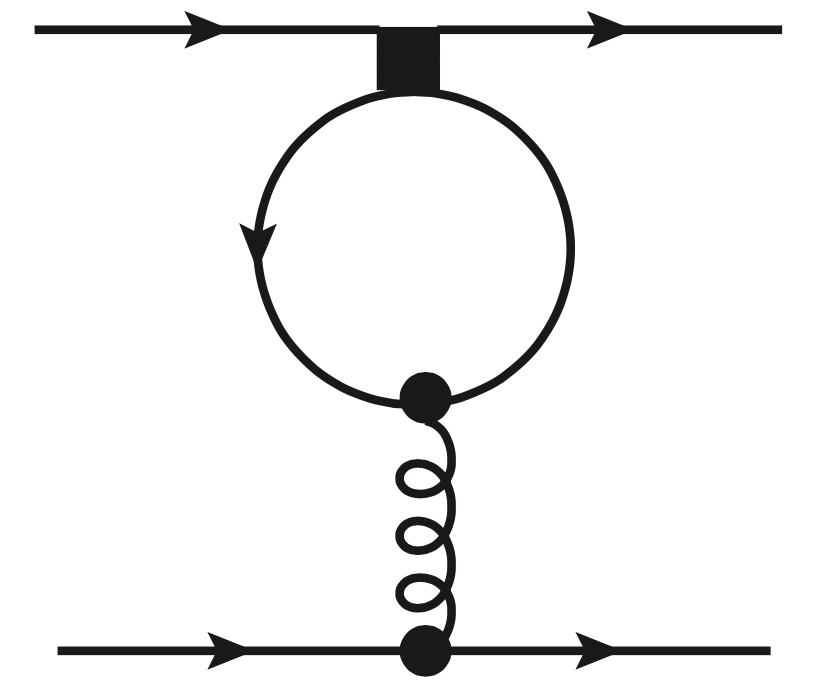
\includegraphics[width=0.4\textwidth]{penguinDiagram.jpg}
\caption{Exemplary one-loop penguin diagram that have to be calculated within the V+A case.}
\label{fig:penguinDiagram}
\end{figure}
As we will see there exists another possible penguin contraction, which we want to introduce to a later point of time. To get an useful, more general, relation we want to start computing the penguin diagram appearing from the singlet vector operator $Q^S_V$. Later we will see, that the singlet axialvector, the octet vector and the octet axial contributions can be easily constructed from the singlet vector penguin contribution. Hence for our desired penguin diagram 
	\begin{equation}
		\begin{split}
			\Gamma^{S(1)} &= - g_s^2 \int d^dx_1 d^dx_2 d^dx_3 d^dx_4 d^dy_1 d^d y_2 d^d z e^{i(p_1x_1 + p_2x_2 + p_3x_3 + p_4x_4)} \\	
			& \cdot  \langle 0  | \{ q^i_\alpha (x_1) \bar q^j_\beta (x_2) [ \bar q^A \gamma_1 q^B \bar q^B \gamma_2 q^A ] (z) \sum_q [\bar q \gamma^\lambda t^b b^b_\lambda q ] (y_1) \sum_q [\bar q \gamma^\sigma t^c b^c_\sigma q ] (y_2) q^k_\delta (x_3) \bar q^j_\gamma (x_4) \}  | 0  \rangle \\				
			&= ig_s^2 [S^A(x_1-z) \gamma_1 S^B(z-y_1) \gamma^\lambda t^b S^B(y_1-z) \gamma_2 S^A(z-x_2)]_{\alpha\beta} \delta^{bc} D_{\lambda\sigma} (y_1 - y_2) \\
			&\cdot \sum_q [S^q(x_3 - y_2) \gamma^\sigma t^c S^q(y_2 - x_4)]_{\delta\gamma} \\
			 &= ig^2_s \mu^{2\epsilon} \int \frac{d^dk}{(2\pi)^d} [S^A(p_1) \Gamma_1 S^B(p_1+k) \gamma^\lambda t^b S^B(-p_2 + k) \Gamma_2 S^A(-p_2)]_{\alpha\beta} \\
			&\cdot \sum_q [S^q(p_3) \gamma^\sigma t^b S^q(-p_4) ]_{\delta\gamma} D_{\lambda\sigma}(p_1+p_2) .
		\end{split}	
	\end{equation}
	Amputating the external quark-propagators and plugging in the non-external ones yields
	\begin{equation}	
		\begin{split}
			\Gamma^{S(1)}_{amp} &= i g^2_s \mu^{2\epsilon} \int \frac{d^dk}{(2\pi)^d} [\Gamma_1 S^B(p_1+k) \gamma^\lambda t^b S^B(-p_2+k) \Gamma_2]^{AB}_{\alpha\beta} \sum_q [\gamma^\sigma t^b]^{q q}_{\delta\gamma} D_{\lambda \sigma (p_1 + p_2)} \\
			 &= - ig^2_s \mu^{2 \epsilon} \int \frac{d^D s}{(2 \pi)^D} [\Gamma_1 S^B(p-s) \gamma^\lambda t^b S^{B}(-s) \Gamma_2 ]^{AB}_{\alpha\beta} \sum_q [\gamma^\sigma t^b ]^{q q} D_{\lambda\sigma}(p) \\
			&= i g^2_s \mu^{2\epsilon} \int \frac{d^Ds}{(2\pi)^D} \frac{s_\mu (p-s)_\nu}{s^2 (p-s)^2} [\Gamma_1 \gamma^\nu \gamma^\lambda \gamma^\mu \Gamma_2 t^b]^{AB}_{\alpha\beta} \sum_q [ \gamma^\sigma t^b ]^{q q}_{\delta\gamma} [-g_{\lambda\sigma} + (1-a) \frac{p_\lambda p_\sigma}{p^2}]\frac{1}{k^2}, 
		\end{split}
	\end{equation}
	where we performed the substitution $p\equiv p_1+p_2$ and $s\equiv p_2 -k$. The appearing integral is given by 
	\begin{equation}
		\int \frac{d^Ds}{(2\pi)^D} \frac{s_\mu (p-s)_\nu}{s^2(p-s)^2} = \frac{i}{(4\pi)^2} \left(\frac{4\pi \mu^2}{-p^2}\right)^\epsilon \frac{\Gamma(2-\epsilon)^2}{\Gamma(4-2\epsilon)} \Gamma(\epsilon) \left[\frac{p^2}{2(1-\epsilon)}g_{\mu\nu} + p_\nu p_\mu \right].
	\end{equation}
	Now employing this result for $\Gamma_1 = \Gamma_2 = \gamma_\mu$ yields 
	\begin{equation}
		\begin{split}
			\label{eq:penguin1Contraction}
			\Gamma^{Q^S_V}_{amp} &= -\frac{g^2_s}{(4\pi)^2} \left(\frac{4\pi \mu^2}{-p^2}\right)^\epsilon \frac{\Gamma(2-\epsilon)^2}{\Gamma(4-2\epsilon)} \Gamma(\epsilon) 4(1-\epsilon) \left\{ [ \gamma_\lambda t^a ]^{AB}_{\alpha\beta} \sum_q [ \gamma_\lambda t^a ]^{qq}_{\delta\gamma} - \frac{[p\!\!\!/ t^a]^{AB}_{\alpha\beta} \sum_q [p\!\!\!/ t^a]^{qq}_{\delta\gamma}}{p^2}\right\} \\
			&= -\frac{a_s}{6} \left[\frac{1}{\hat \epsilon} - ln \left(\frac{-p^2}{\mu^2}\right) + \frac{2}{3} + \mathcal{O}(\epsilon) \right] \left\{ \left[ \gamma^\lambda t^b \right]^{\bar uu} \sum_q \left[ \gamma_\lambda t^b \right]^{\bar qq} + \frac{\left[p\!\!\!/ t^b\right]^{\bar uu} \left[p\!\!\!/ t^b\right]^{\bar qq}}{p^2}\right\},
		\end{split}
	\end{equation}
	where we used lst.~(\ref{lst:MathematicaPenguin1}).
	For insertion of $\Gamma_1=\Gamma_2=\gamma_\mu\gamma_5$ we get the same result. This demonstrates the vanishing penguin diagram contribution of the V-A case! Hence for the V+A case we get twice the contribution. Regarding only the divergent term leads to
	\begin{equation}
		\Gamma^{Q^S_{V+A}}_{amp} = - \frac{a_s}{3}\frac{1}{\hat \epsilon} \left[ [\gamma_\lambda t^a]^{\bar uu} [\gamma^\lambda t^a]^{\bar qq} - [p\!\!\!/ t^a]^{\bar uu} [p\!\!\!/ t^a]^{\bar qq} \frac{1}{p^2} \right] + \mathcal{O}(1).
	\end{equation}
	As we are only interested in the mixing into local operators we will neglect the impulse dependent terms. Thus we can write
	\begin{equation}
		\Gamma^{Q^S_{V+A}}_{amp}(local) = - \frac{a_s}{3}\frac{1}{\hat \epsilon} \left[ [\gamma_\lambda t^a]^{\bar uu} [\gamma^\lambda t^a]^{\bar qq}  \right] + \mathcal{O}(1).
	\end{equation}
	\par
	Coming back to the Q1-octet-mixing contribution we just have to adjust the former penguin diagram with a substitution of 
	\begin{equation}
		t^a \rightarrow t^at^bt^a = -\frac{1}{2N_c},
	\end{equation}
	simply yielding another prefactor. Hence for our penguin diagram we get
	\begin{equation}
		\Gamma^{Q^O_{V+A}}_{amp} = \frac{1}{6N_c} \frac{a_s}{\epsilon} \left\{\left[\gamma_\mu t^a\right]^{\bar uu} + \left[\gamma_\mu t^a\right]^{\bar dd} \right\} \sum_q \left[\gamma^\mu t^a \right]^{\bar qq}.
	 \end{equation}
	\par
	In our former penguin diagram calculation we contracted the $\bar uu$ quark fields. The $\bar dd$ is another possible contraction with the same contribution. Hence its corresponds to a mixing into another operator Q3 	
	\begin{equation}
		Q_3 = (\bar u\gamma_\mu t^a u + \bar d \gamma_\mu t^a) \sum_{q=u,d,s} (\bar q \gamma^\mu t^a q).  	
	\end{equation}
	As before we can now easily read of the renormalization constant
	\begin{equation}
		Z_{13} = \frac{1}{6N_c}. 
	\end{equation}
	Hence we get for the anomalous dimension matrix the additional entry
	\begin{equation}
		\gamma_{13} = -\frac{1}{3 N_c}.
	\end{equation}
	and for the total anomalous row
	\begin{equation}
		\gamma_{Q1} = 
		\begin{pmatrix}
			-\frac{3}{N_c} & \frac{3C_F}{2N_c} & - \frac{1}{3N_c} & 0 & 0 & 0 & 0 & 0 & 0
		\end{pmatrix}
	\end{equation}

	\subsection*{Q2 mixing}
	For the Q2 operator 
	\begin{equation}
		Q_2 = Q^S_V + Q^S_A = \bar u \gamma_\mu d \bar d \gamma_\mu u + \bar u \gamma_\mu \gamma_5 d \bar d \gamma_\mu \gamma_5 u
	\end{equation}
	we can as in the Q1 mixing use our former results. Noticing that Q2 is $Q^S_-$ alike, we get from the current-current diagrams 
	\begin{equation}
		Q^S_V + Q^S_A \rightarrow Q^O_A + Q^O_V \qquad	\Rightarrow \qquad Q^S_+ \rightarrow \frac{3}{2} Q^O_+.
	\end{equation}
	\begin{equation}
		\Gamma^{Q^S_{V+A}} = \frac{a_s}{\epsilon} \frac{3}{2} Q^O_{+} 
	\end{equation}
	Hence for the renormalization constant and the anomalous dimension we get
	\begin{equation}
		Z_{21} = \frac{3}{2} \qquad \text{and} \qquad \gamma_{21} = -3.
	\end{equation}
	As for the Q1 mixing we also we also get a penguin contribution
	\begin{equation}
		\Gamma^{Q^S_+}_{pen} = -\frac{1}{3} \frac{a_s}{\epsilon}.
	\end{equation}
	Thus the contributions lead to 
	\begin{equation}
		Z_{23} = -\frac{2}{6} \qquad \text{and} \qquad \gamma_{23} = \frac{2}{3}.
	\end{equation}
	For the total Q2 mixing we get 
	\begin{equation}
		\gamma_{Q2} = 
		\begin{pmatrix}
			3 & 0 & \frac{2}{3} & 0 & 0 & 0 & 0 & 0 & 0
		\end{pmatrix}
	\end{equation}

	\subsection*{Q3 mixing}
	Due to the similarity of the Q3 operator
	\begin{equation}
		Q_3 = (\bar u\gamma_\mu t^a u + \bar d \gamma_\mu t^a) \sum_{q=u,d,s} (\bar q \gamma^\mu t^a q).  	
	\end{equation}
	to the singlet vector operator we get a contribution from the current-current diagrams of
	\begin{equation}
		\sum_{a,\ldots,f} \Gamma_i = \frac{a_s}{\epsilon} \left[\frac{3N_c}{8}Q_3 - \frac{3C_F}{4N_c}Q_6 - \frac{3}{4}\left(\frac{N_c}{2} - \frac{2}{N_c}\right)Q_4 \right]
	\end{equation}
	As before we also have to regard the penguin contraction, but besides the penguin contraction we already have been calculating in subsec.~(\ref{subsec:Q1Mixing}), we also require a different penguin contraction given by
\begin{equation}	
		\Gamma^{(2)}_{pen} =
%		-------------------------
		\contraction{}{q}{(x_1) \bar q(x_2) [\bar}{q}
		\bcontraction{q(x_1) \bar}{q}{(x_2) [\bar q}{q}
		\bcontraction[2ex]{q(x_1) \bar q(x_2) [\bar q q \bar}{q}{q](z) q(x_3) \bar q(x_4) [B \bar q}{q}
		\bcontraction{q(x_1) \bar q(x_2) [\bar q q \bar q}{q}{](z) q(x_3) \bar q(x_4) [B \bar}{q}
		\contraction[3ex]{q(x_1) \bar q(x_2) [\bar q q \bar q q](z)}{q}{(x_3) \bar q(x_4) [B \bar q q](y_1) [B \bar}{q}
		\contraction[2ex]{q(x_1) \bar q(x_2) [\bar q q \bar q q](z) q(x_3) \bar}{q}{(x_4) [B \bar q q](y_1) [B \bar q}{q}
		\contraction{q(x_1) \bar q(x_2) [\bar q q \bar q q](z) q(x_3) \bar q(x_4) [}{B}{\bar q q](y_1) [}{B}
% 		---------------------------------
		q(x_1) \bar q(x_2) [\bar q q \bar q q](z) q(x_3) \bar q(x_4) [B \bar q q](y_1) [B \bar q q](y_2),
\end{equation}
	where we once again only displayed the fields we wanted to contract. Hence for the second type of penguin diagrams we get the following contribution
	\begin{equation}
		\begin{split}
			\label{eq:penguin2}
			\Gamma^{(2)}_{pen} &= -g^2_s Tr[t^at^b] \mu^{2\epsilon} \int\frac{d^Ds}{(2\pi)^D} Tr[S(p-s)\gamma^\lambda S(-s)\Gamma_2] D_{\lambda \sigma} (p) [\Gamma_1t^a]^{\bar uu} [\gamma^\sigma]^{\bar qq} \\
			&= -\frac{i}{2} g^2_s [\Gamma_1t^a]^{\bar uu} [\gamma^\sigma]^{\bar qq} \mu^{2\epsilon} \int \frac{d^Ds}{(2\pi)^D} \frac{s_\alpha(p-s)_\beta}{s^2(p-s)^2} Tr[\gamma^\beta \gamma^\lambda \gamma^\alpha \Gamma_2] [g_{\lambda\sigma} -(1-a)\frac{p_\lambda p_\sigma}{p^2} ]\frac{1}{p^2} 
		\end{split}.
	\end{equation}
	For the vector case $\Gamma_1 = \Gamma_2 = \gamma_\mu$ we get the same singularity as for the other penguin contraction eq.~(\ref{eq:penguin1Contraction}). Only the finite parts are different
	\begin{equation}
		\begin{split}
			\Gamma^O_{V, pen} &= -\frac{g^2_s}{(4\pi)^2} \left(\frac{4\pi\mu^2}{-p^2}\right)^{\epsilon} \frac{\Gamma^2(2-\epsilon)}{\Gamma(4-2\epsilon)} \Gamma(\epsilon) 4  \left\{ [\gamma_\mu t^a]^{\bar uu} [\gamma^\mu t^a]^{\bar qq} - [p\!\!\!/ t^a]^{\bar uu} [p\!\!\!/ t^a]^{\bar qq} \frac{1}{p^2} \right\} \\
			&= -\frac{a_s}{6} \left\{ \frac{1}{\hat \epsilon} - ln\left(-\frac{p^2}{\mu^2}\right) + \frac{5}{3} + \mathcal{O}(\epsilon) \right\} \left\{ [\gamma_\mu t^a]^{\bar uu} [\gamma^\mu t^a]^{\bar qq} - [p\!\!\!/ t^a]^{\bar uu} [p\!\!\!/ t^a]^{\bar qq} \frac{1}{p^2} \right\}
		\end{split}.
	\end{equation}
	\par
	Having found the singularities of the two appearing penguin diagrams we still have three different possibilities of contracting the gluon-vertex. Starting with the first we want to contract one of the gluon vertexes with the sum of $\bar qq$ 
	\begin{equation}
		\Gamma_{\bar qq} = 
		\contraction[2ex]{}{q}{(x_1) \bar q(x_2) [( \bar u}{q}{}
		\contraction{q(x_1) \bar}{q}{(x_2) [( \bar }{q}{}
		\bcontraction[2ex]{q(x_1) \bar q(x_2) [( \bar u u + \bar d d ) \sum \bar }{q}{q](z) q(x_3) \bar q(x_4) [\sum \bar q}{q}
		\bcontraction{q(x_1) \bar q(x_2) [( \bar u u + \bar d d ) \sum \bar q }{q}{](z) q(x_3) \bar q(x_4) [\sum \bar }{q}
		\contraction[2ex]{q(x_1) \bar q(x_2) [( \bar u u + \bar d d ) \sum \bar q q](z) }{q}{(x_3) \bar q(x_4) [\sum \bar q q](y_1) [\sum \bar }{q}
		\contraction{q(x_1) \bar q(x_2) [( \bar u u + \bar d d ) \sum \bar q q](z) q(x_3) \bar }{q}{(x_4) [\sum \bar q q](y_1) [\sum \bar q}{q}
		q(x_1) \bar q(x_2) [( \bar u u + \bar d d ) \sum \bar q q](z) q(x_3) \bar q(x_4) [\sum \bar q q](y_1) [\sum \bar q q](y_2).
	\end{equation}
	We see that this contraction yields $N_f$ times the contribution of the penguin diagram 
	\begin{equation}
		\Gamma_{\bar qq} = - \frac{a_s}{\epsilon} \frac{N_f}{6} Q_3.
	\end{equation}
	For the second contraction possibility we have a $u\bar u$ contraction of the gluon vertex. Hence
	\begin{equation}
		\Gamma_{\bar uu} = 
		\contraction[2ex]{}{q}{(x_1) \bar q(x_2) [( \bar u u + \bar d d ) \sum \bar }{q}{}
		\contraction{q(x_1) \bar}{q}{(x_2) [( \bar u u + \bar d d ) \sum \bar q }{q}{}
		\bcontraction[2ex]{q(x_1) \bar q(x_2) [( \bar}{u}{u + \bar d d ) \sum \bar q q](z) q(x_3) \bar q(x_4) [\sum \bar q }{q}
		\bcontraction{q(x_1) \bar q(x_2) [( \bar u}{u}{+ \bar d d ) \sum \bar q q](z) q(x_3) \bar q(x_4) [\sum \bar }{q}
		\contraction[2ex]{q(x_1) \bar q(x_2) [( \bar u u + \bar d d ) \sum \bar q q](z) }{q}{(x_3) \bar q(x_4) [\sum \bar q q](y_1) [\sum \bar }{q}
		\contraction{q(x_1) \bar q(x_2) [( \bar u u + \bar d d ) \sum \bar q q](z) q(x_3) \bar }{q}{(x_4) [\sum \bar q q](y_1) [\sum \bar q}{q}
		q(x_1) \bar q(x_2) [( \bar u u + \bar d d ) \sum \bar q q](z) q(x_3) \bar q(x_4) [\sum \bar q q](y_1) [\sum \bar q q](y_2).
	\end{equation}	
	As the gluon vertex contraction of $\bar uu$ we get the same result contracting $d \bar d$ 
	\begin{equation}
		\Gamma_{\bar dd} = -\frac{a_s}{\epsilon}\frac{1}{3} \sum_q (\bar q \gamma_\mu t^a q) \sum_{q'} (\bar q' \gamma^\mu t^a q') = - \frac{a_s}{\epsilon}\frac{1}{3} Q_7.
	\end{equation}
	The final contribution are two cross contractions
	\begin{equation}
		\Gamma_{cross} = 
		\contraction[2ex]{}{q}{(x_1) \bar q(x_2) [( \bar}{u}
		\contraction{q(x_1) \bar}{q}{(x_2) [( \bar u u + \bar d d ) ( \bar u}{u}{}
		\bcontraction{q(x_1) \bar q(x_2) [( \bar u}{u}{+ \bar d d ) ( \bar u u + \bar d d + \bar s s )](z) q(x_3) \bar q(x_4) [\sum \bar }{q}
		\bcontraction[2ex]{q(x_1) \bar q(x_2) [( \bar u u + \bar d d ) ( \bar}{u}{u + \bar d d + \bar s s )](z) q(x_3) \bar q(x_4) [\sum \bar q}{q}
		\contraction[2ex]{q(x_1) \bar q(x_2) [( \bar u u + \bar d d ) ( \bar u u + \bar d d + \bar s s )](z) }{q}{(x_3) \bar q(x_4) [\sum \bar q q](y_1) [\sum \bar }{q}
		\contraction{q(x_1) \bar q(x_2) [( \bar u u + \bar d d ) ( \bar u u + \bar d d + \bar s s )](z) q(x_3) \bar }{q}{(x_4) [\sum \bar q q](y_1) [\sum \bar q}{q}
		q(x_1) \bar q(x_2) [( \bar u u + \bar d d ) ( \bar u u + \bar d d + \bar s s )](z) q(x_3) \bar q(x_4) [\sum \bar q q](y_1) [\sum \bar q q](y_2),
	\end{equation}
	where we also could cross contract the $\bar d d$. Hence the contribution is denoted by
	\begin{equation}
		\bar u \gamma_\mu t^a u t^b \gamma^\lambda \bar u \gamma^\mu t^a u + \bar d \gamma_\mu t^a d t^b \gamma^\lambda \bar d \gamma^\mu t^a d, 
	\end{equation}
	yielding
	\begin{equation}
		\Gamma_{cross} = -\frac{a_s}{\epsilon} \frac{1}{N_c} \frac{1}{6} Q_3.
	\end{equation}
	Multiplying every piece by -2 yields the third row of the anomalous dimension matrix $\hat \gamma^{(1)}$ entries (the $Q_3$ mixing) 
	\begin{equation}
		\gamma_{Q3} = 
		(
		\begin{matrix}
			0 & 0 & -\frac{3N_c}{4}+\frac{N_f}{3}-\frac{1}{3N_c} & \frac{3N_c}{4} - \frac{3}{N_c} & \frac{3C_F}{2 N_c} & \frac{2}{3} & 0 & 0 & 0
		\end{matrix}.
		)
	\end{equation}

	\subsection*{Q4 Mixing}
	As the procedure of finding the entries for the anomalous dimension matrix is going to repeat with ever mixing we will only go back into details if they are needed. For the Q4 mixing
	\begin{equation}
		Q_4 = (\bar u \gamma_\mu \gamma_5 t^a u + \bar d \gamma_\mu \gamma_5 d) \sum_{q=u,d,s} (\bar q \gamma^\mu \gamma_5 t^a q)
	\end{equation}
	we get the current-current diagram contribution
	\begin{equation}
		\sum_{i=a,\ldots,f}\Gamma_i = \frac{a_s}{\epsilon}\left[\frac{3N_c}{8}Q_4 -\frac{3C_F}{4N_c}Q_5 -\frac{3}{4}\left(\frac{N_c}{2}-\frac{2}{N_c}\right)Q_3\right].
	\end{equation}
	Noticing that we have a mixing into the operator Q5. Q5 is in general an basic operator. However, in four dimensions, one operator in the full set is redundant and can be expressed through the others by means of Fierz transformations yielding the relation
	\begin{equation}
		Q_2 = \frac{\left(2Q_1 + 2Q_3 + 2Q_4 -\left(1-\frac{1}{N_c}\right)(Q_5 + Q_6)- Q_7 -Q_8 -\left(1-\frac{1}{N_c}\right)\left(\frac{Q_9 + Q_{10}}{2}\right)\right)}{1-\frac{1}{N_c}}.
	\end{equation}
	Using Mathematica lst.~(\ref{lst:MathematicaQ4Mixing}) we can solve for Q5 and substitute $C_F$ through its $N_c$ dependencies, giving us the input of the normal diagrams. Adding as well the contribution of the penguin diagrams
	\begin{equation}
		\Gamma_{cross} = \frac{a_s}{\epsilon} \frac{1}{6N_c} Q_3
	\end{equation}
	will give us the total input of the divergencies 
	\renewcommand{\arraystretch}{2.5}
	\begin{equation}
		\begin{array}{c | c | c}
			\Gamma_{Q_1} = -\frac{3}{4N_c} - \frac{3}{4} &  \Gamma_{Q_2} = \frac{3C_F}{4N_c}, & \Gamma_{Q_3} = -\frac{3}{4} -\frac{3N_c}{8} + \frac{11}{12N_c},\\ 
			\hline
			 \Gamma_{Q_4} = -\frac{3}{4N_c} -\frac{3}{4} + \frac{3N_c}{8}, & \Gamma_{Q_6} = \frac{3C_F}{4N_c}, & \Gamma_{Q_7} = \frac{3}{8N_c} + \frac{3}{8}, \\
			\hline
			\Gamma_{Q_8} = \frac{3}{8N_c} + \frac{3}{8}, & \Gamma_{Q_9} = \frac{3C_F}{8N_c}, & \Gamma_{Q_{10}} = \frac{3C_F}{8N_c}.
		\end{array}
	\end{equation}
	\renewcommand{\arraystretch}{1}
	Hence for the anomalous dimension we get 
	\begin{equation}
		\gamma_{Q4} = 
		\left(
		\begin{matrix}
			0 & 0 & \frac{N_f}{3}-\frac{3N_c}{4}-\frac{1}{3N_c} & \frac{3N_c}{4}-\frac{3}{N_c} & -\frac{3C_F}{2N_c} & -\frac{3}{4}-\frac{3}{4N_c} & -\frac{3}{4}-\frac{3}{4N_c} & \frac{3C_F}{4N_c} & \frac{3C_F}{4N_c} \\
		\end{matrix}
		\right)
	\end{equation}
	As we substituted the redundant operator $Q_5$ we will directly continue with $Q_6$.

	\subsection*{Q6 Mixing}
	The Q6 operator is given by
	\begin{equation}
		Q_6 = ( \bar u \gamma_\mu \gamma_5 u + \bar d \gamma_\mu \gamma_5 d )\sum (\bar q \gamma^\mu \gamma_5  q).
	\end{equation}
	Using former results we get 	
	\begin{equation}
		\sum_{i=a,...,f} \Gamma_i = -\frac{a_s}{\epsilon}\frac{3}{2}Q_3
	\end{equation}
	for the current-current diagrams. For the penguin contribution we only regard the first type of of penguin contractions. The Q6 operator has no octet structure and consequently the trace $Tr[t^at^bt^a]$ in eq.~(\ref{eq:penguin2}) is going to vanish. Hence we only get an additional contribution of
	\begin{equation}
		\Gamma_{pen} = -\frac{a_s}{\epsilon}\frac{1}{3}Q_3
	\end{equation}
	and in total for the $\hat \gamma$ matrix
	\begin{equation}
		\gamma_{Q_6} =
		\begin{pmatrix}
			0 & 0 & \frac{11}{3}Q_3 & 0 & 0 & 0 & 0 & 0 & 0 
		\end{pmatrix}
	\end{equation}
	
	\subsection*{Q7 Mixing}
	The $Q_7$ operator is given by
	\begin{equation}
		\sum_{q=u,d,s} ( \bar q \gamma_\mu t^a q ) \sum_{q'=u,d,s} (\bar q' \gamma^\mu t^a q'),
	\end{equation}
	yielding the contributions
	\begin{equation}
	\frac{a_s}{\epsilon} \left[\frac{3N_c}{8}Q_7 - \frac{3C_F}{4N_c}Q_{10} - \frac{3}{4}\left(\frac{N_c}{2}-\frac{2}{N_c}\right)\right]
	\end{equation}
	and
	\begin{equation}
		\Gamma^{Q_7}_{q\bar q} = \frac{a_s}{\epsilon}\frac{N_f}{6}Q_7, \qquad \Gamma^{Q_7}_{\bar uu} = -\frac{a_s}{\epsilon} \frac{1}{2} Q_7, \qquad \Gamma^{Q_7}_{cross} = \frac{a_s}{\epsilon} \frac{1}{6N_c} Q_7.
	\end{equation}
	Consequently we get
	\begin{equation}
		\gamma_{Q7} = 
		\begin{pmatrix}
			0 & 0 & 0 & 0 & 0 & \frac{N_f}{3}+1-\frac{3N_c}{4}-\frac{1}{3N_c} & -\frac{3}{4}-\frac{3}{4N_c} & \frac{3C_F}{4N_c} & \frac{3C_F}{4N_c}
		\end{pmatrix}
	\end{equation}
	
	\subsection*{Q8 Mixing}
	Q8 is given by
	\begin{equation}
		Q_8 = \sum_{q=u,d,s}(\bar q \gamma_\mu \gamma_5 t^a q) \sum_{q'=u,d,s} (\bar q' \gamma^\mu \gamma_5 t^a q).
	\end{equation}
	Hence we get the following contributions
	\begin{equation}
		\sum_{i=a,\ldots,f} \Gamma_i = \frac{a_s}{\epsilon} \left[ \frac{3N_c}{8}Q_8 - \frac{3C_F}{4N_c}Q_9 - \frac{3}{4}\left(\frac{N_c}{2}-\frac{2}{N_c}\right)Q_7 \right]
	\end{equation}
	for the current-current diagrams and
	\begin{equation}
		\Gamma^{Q_8}_{cross} = \frac{a_s}{\epsilon} \frac{1}{6N_c}Q_7
	\end{equation}
	for the penguin ones. The two additional contributions from the $\bar qq$ and $\bar uu$ contraction we applied do not exist. The additional $\gamma_5$ matrix let the trace appearing in eq.~(\ref{eq:penguin2}) disappear for an odd number of $\gamma$ matrices. Hence in total we get for the anomalous dimension a contribution of
	\begin{equation}
		\gamma_{Q8} = 
		\begin{pmatrix}
			0 & 0 & 0 & 0 & 0 & \left(\frac{3N_c}{4}-\frac{10}{3N_c}\right) & -\frac{3N_c}{4} & + \frac{3C_F}{2N_c} 			
		\end{pmatrix}
	\end{equation}

	\subsection*{Q9 Mixing}
	The Q9 operator is given by
	\begin{equation}
		Q_9 = \sum_{q=u,d,s}(\bar q \gamma_\mu q) \sum_{q'=u,d,s}(\bar q' \gamma^\mu q')
	\end{equation}
	and gives us the contributions
	\begin{equation}
		\sum_{i=a,\ldots,f} \Gamma_i = -\frac{a_s}{\epsilon} \frac{3}{2}Q_8 \qquad \text{and} \qquad cross_{Q_9} - \frac{a_s}{\epsilon} \frac{1}{3} Q_7
	\end{equation}
	Hence in total
	\begin{equation}
		\gamma_{Q9} = 
		\begin{pmatrix}
			0 & 0 & 0 & 0 & 0 & \frac{2}{3} & 3 & 0 
		\end{pmatrix}.
	\end{equation}
	
	\subsection*{Q10 Mixing}
	Our final operator is given by
	\begin{equation}
		Q_{10} = \sum_{q=u,d,s}(\bar q \gamma_\mu \gamma_5 q) \sum_{q'=u,d,s} (\bar q' \gamma^\mu \gamma_5 q')
	\end{equation}
	contributing with the factors
	\begin{equation}
		\sum_{i=a,\ldots,f} \Gamma_i = -\frac{a_s}{\epsilon} \frac{3}{2} Q_7 \qquad \text{and} \qquad \Gamma^{Q_{10}}_{pen} = -\frac{a_s}{\epsilon} \frac{1}{3} Q_7.
	\end{equation}
	Hence for our anomalous dimension matrix we get
	\begin{equation}
		\gamma_{Q10} =
		\begin{pmatrix}
			0 & 0 & 0 & 0 & 0 & \frac{11}{3} & 0 & 0 & 0  
		\end{pmatrix}
	\end{equation}

	\subsection{V+A Anomalous Dimension Matrix}	
	Putting all former factors from the operator mixing together we get our desired matrix for the anomalous dimension.
	\begin{equation}
		\begin{split}
			\label{eq:anomalousDimensionMatrixVpA}
			\gamma^{(1)}_{Q_+} &= 
			\left(\begin{matrix}
				-\frac{3}{N_C} & \frac{3C_F}{2N_C} &-\frac{1}{3N_C} & 0   
				\\
				3 & 0 & \frac{2}{3} & 0    \\
				0 & 0 & \frac{N_f}{3}-\frac{3N_c}{4}-\frac{1}{3N_c} & \frac{3N_c}{4}-\frac{3}{N_c}   \\
				\frac{3}{2}+\frac{3}{2N_c} & -\frac{3C_F}{2N_c} & \frac{3N_c}{4}+\frac{3}{2}-\frac{11}{6N_c} & -\frac{3N_c}{4}+\frac{3}{2}+\frac{3}{2N_c} \\
				0 & 0 & \frac{11}{3} & 0 \\
				0 & 0 & 0 & 0 \\
				0 & 0 & 0 & 0 \\
				0 & 0 & 0 & 0 \\
				0 & 0 & 0 & 0 
			\end{matrix} \right. \\
			&\qquad\qquad\qquad\qquad\qquad\qquad \left.\begin{matrix}
				0 & 0 & 0 & 0 & 0 \\
				0 & 0 & 0 & 0 & 0 \\
				\frac{3C_F}{2N_C} & \frac{2}{3} & 0 & 0 & 0 \\
				-\frac{3C_F}{2N_c} & -\frac{3}{4}-\frac{3}{4N_c} & -\frac{3}{4}-\frac{3}{4N_c} & \frac{3C_F}{4N_c} & \frac{3C_F}{4N_c} \\
				0 & 0 & 0 & 0 & 0 \\
				0 & \frac{N_f}{3}+1-\frac{3N_c}{4}-\frac{1}{3N_c} & \frac{3N_c}{4}-\frac{3}{N_c} & 0  & \frac{3C_F}{2N_c} \\
				0 & \frac{3N_c}{4}-\frac{10}{3N_c} & -\frac{3N_c}{4} & \frac{3C_F}{2N_c} & 0 \\
				0 & \frac{2}{3} & 3 & 0 & 0 \\
				0 & \frac{11}{3} & 0 & 0 & 0 
			\end{matrix}\right)
		\end{split}
	\end{equation}
	\\\\

\section{Confirming RGE}
To check the RGE eq.~(\ref{eq:rgeCheck}) we just have to insert $C^{V-A}_6$ eq.~(\ref{C6O6VmA}), $C^{V+A}_6$ eq.~(\ref{C6O6VpA}) as well as the two former calculated anomalous dimension matrices of the first order, given by eq.~(\ref{eq:anomalousDimensionMatrixVmA}) and eq.~(\ref{eq:anomalousDimensionMatrixVpA}). Furthermore we want to remind that we have to deal with the total derivative of $\mu$ which is given in the RGE eq.~(\ref{eq:RGE}) yielding
\begin{equation}
	\begin{split}
		\mu \frac{d}{d \mu} &= \mu \frac{\partial}{\partial \mu} - \beta(a_s)  \frac{\partial}{\partial a_s}  \\
		&=  \mu \frac{\partial}{\partial \mu} - \beta_1 a_s^2 \frac{\partial}{\partial a_s}, 
	\end{split}
\end{equation}
where we are only interested in the first order, with a give $\beta_1 = (11 N_c - 2N_f)/6$ and neglected the partial derivative of the mass, as we are working in the massless case.

\subsection*{V-A Case}
Starting with the V-A case we used a Mathematica script app.~(\ref{lst:MathematicaCheckOfRGE}). Regarding the output the file confirmed the same structure for the left-hand side and right-hand side of eq.~(\ref{eq:rgeCheck}) we wanted to check for. The both sides are thus given by
\begin{equation}
	6 a^2_s \pi^2 
	\begin{pmatrix}
		\frac{4}{N_c} - 2 N_c \\
		-1 + N_c^{-2}
	\end{pmatrix}
\end{equation}

\subsection*{V+A Case}
For the V+A case we are using the same file and get the approval of eq.~(\ref{eq:rgeCheck}) being fulfilled. The structure of the both equation sides are given by
\begin{equation}
	a^2_s \pi^2
	\begin{pmatrix}
		\frac{24}{N_c} & -6 & \frac{6}{N_c^2} & \frac{88}{27 N_c} + \frac{4 N_c}{3} - \frac{16 N_f}{27} & \frac{16}{3N_c} - \frac{4 N_c}{3} & - \frac{4}{3} + \frac{4}{3N_c^2} & - \frac{32}{27} & 0 & 0 & 0
	\end{pmatrix}
\end{equation} 
